\section{结果}

\subsection{评估地图与核心结果}

第~4 章将穿深 surrogate 定义为一个具备删失感知的低维概率回归问题。因此，本章结果不再组织成单一的排行榜，而是一组相互关联的评估视图。full-clean CDF 协议在 Dataset~\#1 的所有已清洗留出 CDF 点上测试部署的逐点 surrogate。uncensored CDF 表是 Dataset~\#2 中主要的删失控制逐点检查。P50-observed 和 q1-extrapolated 表是工况级检查，用于分离窗口内的代表性行为与外推延续行为。留一喷嘴族（LONO）协议测试对未见喷嘴族的转移能力，最后的消融部分则对使 MLP 能够用于下游筛查工作流的各项设计选择进行归因。

提取与拟合工作流在已处理的 campaign 归档中生成了 295 个清洗后的拟合轨迹文件。这一步之所以重要，是因为 surrogate 并不是直接训练在原始且间歇性断裂的 plume 轨迹上，而是训练在保留主要时间结构、同时削弱分割噪声并降低晚期删失偏差的目标上。图~\ref{fig:clean-fit-example} 给出一个代表性例子：清洗后的曲线保留了 plume-to-plume 的差异，而拟合轨迹则提供了平滑且仍忠于观测液相包络的删失感知目标。

\begin{figure}[t]
\centering
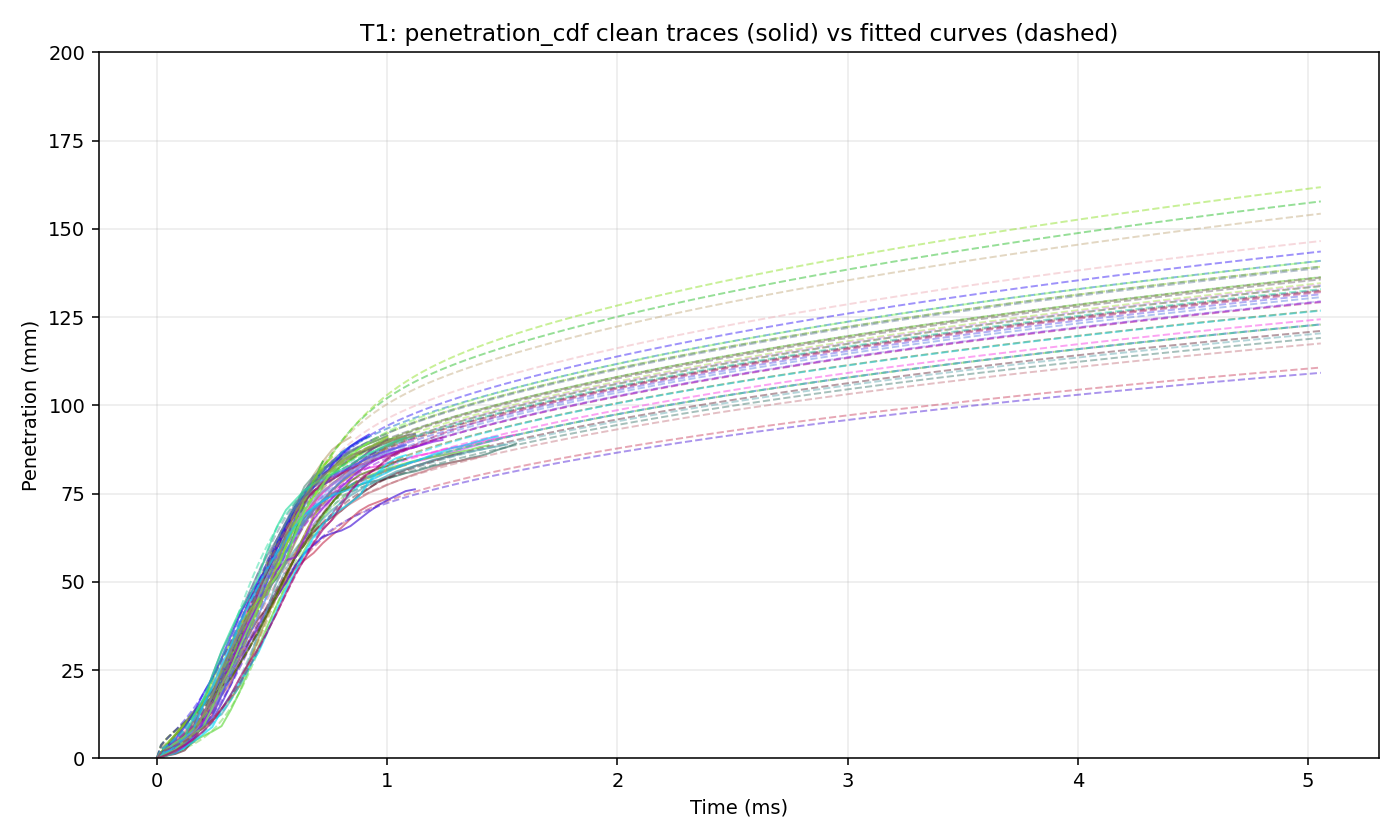
\includegraphics[width=0.92\linewidth]{images/representative_clean_fit.png}
\caption{BC20241003\_HZ\_Nozzle1 campaign 中 T24 工况的清洗后轨迹与 q1 拟合曲线（\textbf{清洗后的 CDF 穿深}）。实线表示逐帧的原始穿深观测，虚线为对应的 $t^{1/4}$ 单支（q1）拟合曲线。该工况包含数十条喷油束轨迹，可清晰看到 plume-to-plume 的差异与拟合的延续行为；拟合曲线在观测结束后平滑外推至 $\SI{3}{ms}$，为后续 surrogate 训练提供了具备删失感知的目标。}
\label{fig:clean-fit-example}
\end{figure}

\subsection{域内 CDF 精度与不确定度}

表~\ref{tab:model-summary} 总结了三个学习阶段的作用和留出集表现。Stage~1 在每个工况只使用一条代表性曲线进行训练，充当稳定的均值锚点；其测试 MAE 为 \SI{2.91}{mm}，在对应的代表性测试集上测得。Stage~2 解决的是更困难的任务——在完整过滤归档上跨越工况内的 plume-to-plume 差异并学习条件方差；其测试 MAE 为 \SI{5.63}{mm}，是在更大、更异质的测试群体上度量的。两组数字因此并不直接可比：较高的 Stage~2 MAE 反映的是更难的监督目标，而非精度下降，这也使得 Stage~2 成为合适的不确定性感知教师模型。

在刷新后的全净化 CDF 评估协议下，采用生产蒸馏损失形式（均值 MSE 与对数方差 MSE 的混合，方差权重 \(\lambda_\sigma=5.0\)）在五个种子（\(\{7,17,42,99,2024\}\)）上训练的无锚点阶段三模型，在每个种子的 24{,}316 条轨迹、692{,}942 个留出时间点上达到整体 RMSE~\(\SI{4.735}{mm}\pm\SI{0.037}{mm}\)、MAE~\(\SI{3.293}{mm}\pm\SI{0.039}{mm}\) 以及微小的正向偏差~\(\SI{+0.626}{mm}\pm\SI{0.112}{mm}\)。图~\ref{fig:pred-vs-actual-best} 表明，在整个测量范围内，留出集预测基本贴近恒等线，且随着穿深增大，散点逐步变宽。这种变宽与异方差设计是一致的：模型并没有强行对所有时刻和工况使用同一个固定误差条。

不确定度校准在工程上同样有意义。全清洗协议下的最终 5 种子平均 1$\sigma$ 与 2$\sigma$ 覆盖率分别为 86.7\% 和 98.5\%，明显比名义高斯值 68.3\% 和 95.4\% 更保守。图~\ref{fig:stage3-calibration-coverage} 进一步把这一点展开为按预测标准差分箱的可靠性图和覆盖率曲线，而不只比较平均标准差与平均误差。对于早期设计筛查而言，这种保守偏置是一个特性而非缺陷：模型有意比精确校准的高斯分布更谨慎，因此不太容易低估晚期时间或弱观测区间下的穿深不确定度。

\begin{figure}[t]
\centering
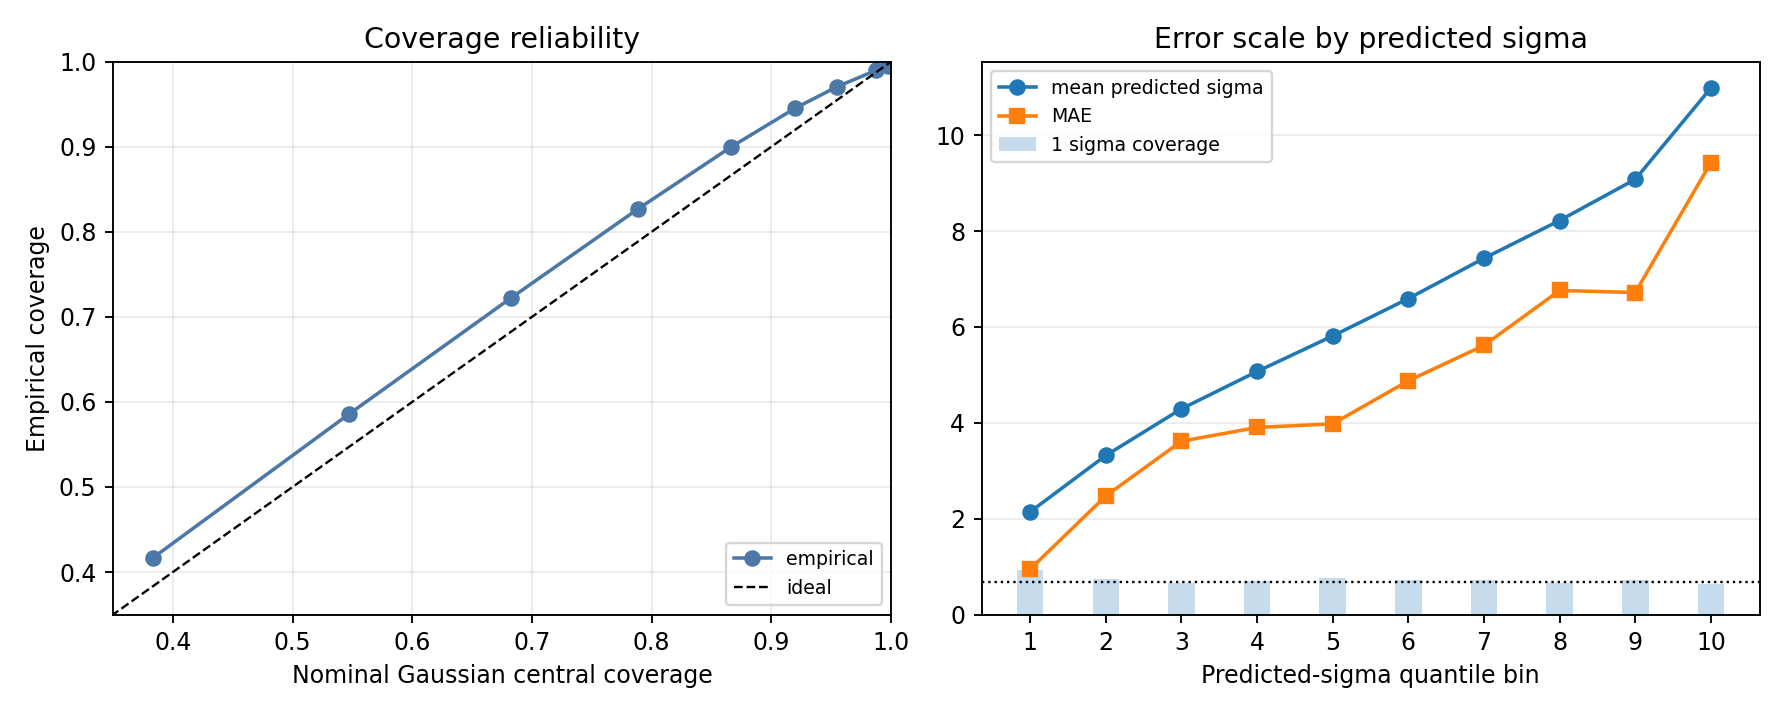
\includegraphics[width=0.94\linewidth]{images/stage3_calibration_coverage.png}
\caption{最终无锚点阶段三模型的不确定度校准检查，由附录~\ref{app:implementation_mapping} 所列的校准覆盖审计脚本从留出集逐点输出重建。图中同时报告按预测 \(\sigma\) 分箱的误差尺度、名义覆盖率曲线，以及平均预测标准差与平均绝对误差的对比。}
\label{fig:stage3-calibration-coverage}
\end{figure}

\begin{table}[t]
\centering
\footnotesize
\setlength{\tabcolsep}{3pt}
\begin{tabular}{@{}L{0.14\linewidth}L{0.22\linewidth}L{0.24\linewidth}L{0.30\linewidth}@{}}
\toprule
阶段 & 监督目标 & 核心留出集指标 & 解释 \\
\midrule
阶段一 & 代表性拟合轨迹（599 行；421/89/89 切分） &
测试 MAE~\SI{2.91}{mm}（生产七特征变体：$\alpha=0.5$ 带压力残差） &
在 7 特征设计并经过 $A$ 缩放后提供稳定的均值锚点，每个工况一条代表性曲线。 \\
阶段二 & 完整过滤拟合集（49{,}908 训练 / 10{,}961 验证 / 10{,}831 测试轨迹） &
测试 MAE~\SI{5.63}{mm}；平均预测标准差~\SI{7.61}{mm}；验证 NLL~$-0.323$ &
更困难的教师任务：在完整过滤归档上把条件均值与条件离散度分开学习。 \\
阶段三 & 带区制相关 KD 引导的原始 CDF，均值与对数方差混合 MSE 蒸馏损失（\(\lambda_\sigma=5.0\)），无锚点 &
全净化 5 种子均值：RMSE~\(\SI{4.735}{mm}\pm\SI{0.037}{mm}\)；MAE~\(\SI{3.293}{mm}\pm\SI{0.039}{mm}\)；偏差~\(\SI{+0.626}{mm}\pm\SI{0.112}{mm}\)；覆盖率 86.7\% / 98.5\% &
生产无锚点筛查模型，具有更好的早期保真度和保守的晚期行为；最终核心指标见下方的外部清洗协议。 \\
\bottomrule
\end{tabular}
\caption{三阶段 surrogate 训练及其在最终筛查工作流中的作用。}
\label{tab:model-summary}
\end{table}

\begin{figure}[t]
\centering
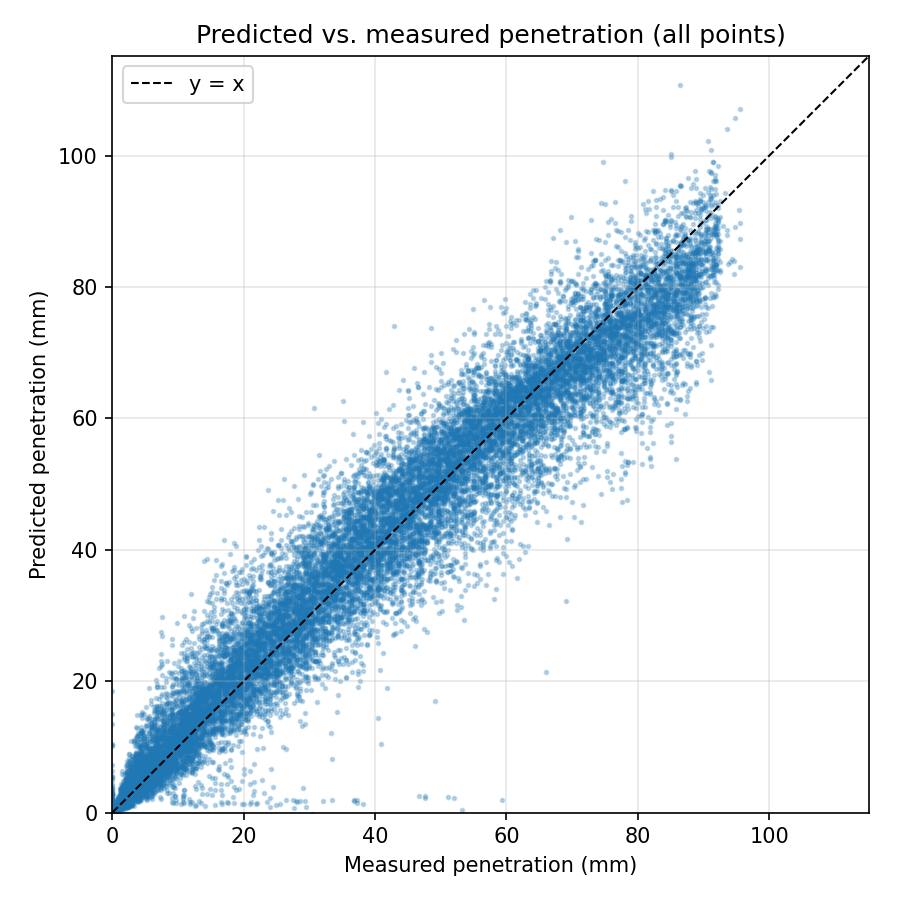
\includegraphics[width=0.88\linewidth]{images/neural_network_fit_results/pred_vs_actual_best.png}
\caption{最终 Stage~3 模型在全部留出集点上的预测穿深与测量穿深对比。虚线表示理想一致线。}
\label{fig:pred-vs-actual-best}
\end{figure}

上述留出集结果反映了阶段三在最初归档训练与评估单一切分下的表现。为了检验结论是否依赖该单一切分，本文进一步引入一个外部清洗评估协议。刷新后的全净化 CDF 协议包含 692{,}942 个预测点和 24{,}316 条轨迹，所有模型都在同一目标集合上进行评估。表~\ref{tab:external-clean-headline} 汇总了物理基线、生产 MLP 变体以及阶段三稀疏异方差高斯过程（SVGP）替代主干：校准后的 Hiroyasu--Arai 经验关联式、带延迟项的 Naber--Siebers 关联式、生产多种子 MLP、面向外推正则化的诊断 KD 变体（仅 $\mu$-锚点、不确定区间使用原始 NLL 监督），以及阶段三 SVGP。物理基线的拟合协议见第~\ref{sec:baseline-fitting-protocol-zh} 节，SVGP 的构造见第~\ref{sec:svgp-alternative-backbone-zh} 节。在生产无锚点配置下五次重复训练的平均 RMSE 为 \SI{4.735}{mm}、MAE 为 \SI{3.293}{mm}、P95 绝对误差为 \SI{9.167}{mm}，并给出 0.867/0.985 的保守 1$\sigma$/2$\sigma$ 覆盖率。相对 Hiroyasu--Arai 与 Naber--Siebers，RMSE 分别降低 58.0\% 和 55.1\%。SVGP 在点预测 RMSE/MAE 上仍略优（RMSE \SI{4.628}{mm}），因此当前的结论并不是 MLP 全面压过核主干；而是生产 MLP 在点精度上与之接近、尾部误差相当，并在覆盖率上刻意保持更为保守。随后，预测分布被投影到图~\ref{fig:impingement-preview-zh}--\ref{fig:impingement-summary-zh} 所示的简化二维发动机几何模型上，产生概率性的撞壁筛查代理指标，而非确定性的通过/不通过阈值。

\begin{table}[t]
\centering
\footnotesize
\setlength{\tabcolsep}{3pt}
\begin{tabular}{@{}L{0.28\linewidth}rrrrrr@{}}
\toprule
模型 & RMSE & MAE & Bias & P95 & 1$\sigma$ & 2$\sigma$ \\
\midrule
校准后的 Hiroyasu--Arai & 11.268 & 8.658 & 0.288 & 22.891 & 0.615 & 0.912 \\
带延迟项的 Naber--Siebers & 10.545 & 8.177 & -0.442 & 21.253 & 0.637 & 0.919 \\
三阶段 MLP，生产 anchor-off，五次重复均值 & 4.735 & 3.293 & 0.626 & \textbf{9.167} & 0.867 & 0.985 \\
三阶段 MLP，诊断 KD 变体（$\mu$-锚点，不确定区间原始监督），五次重复均值 & 5.200 & 3.654 & -0.585 & 10.525 & 0.834 & 0.985 \\
稀疏异方差 GP，Stage~3 模式 & \textbf{4.628} & \textbf{3.173} & -0.070 & 9.242 & 0.703 & 0.939 \\
\bottomrule
\end{tabular}
\caption{刷新后的全净化 CDF 评估协议下的扩展结果。误差单位为 mm；P95 为 95\% 绝对误差。两条 MLP 行均为五次重复训练（seeds 7/17/42/99/2024）的均值，SVGP 行为已训练的阶段三 seed-42 参考模型。名义高斯覆盖率约为 0.683 / 0.954。原始数据归档路径详见附录~\ref{app:implementation_mapping}。}
\label{tab:external-clean-headline}
\end{table}

\begin{figure}[t]
\centering
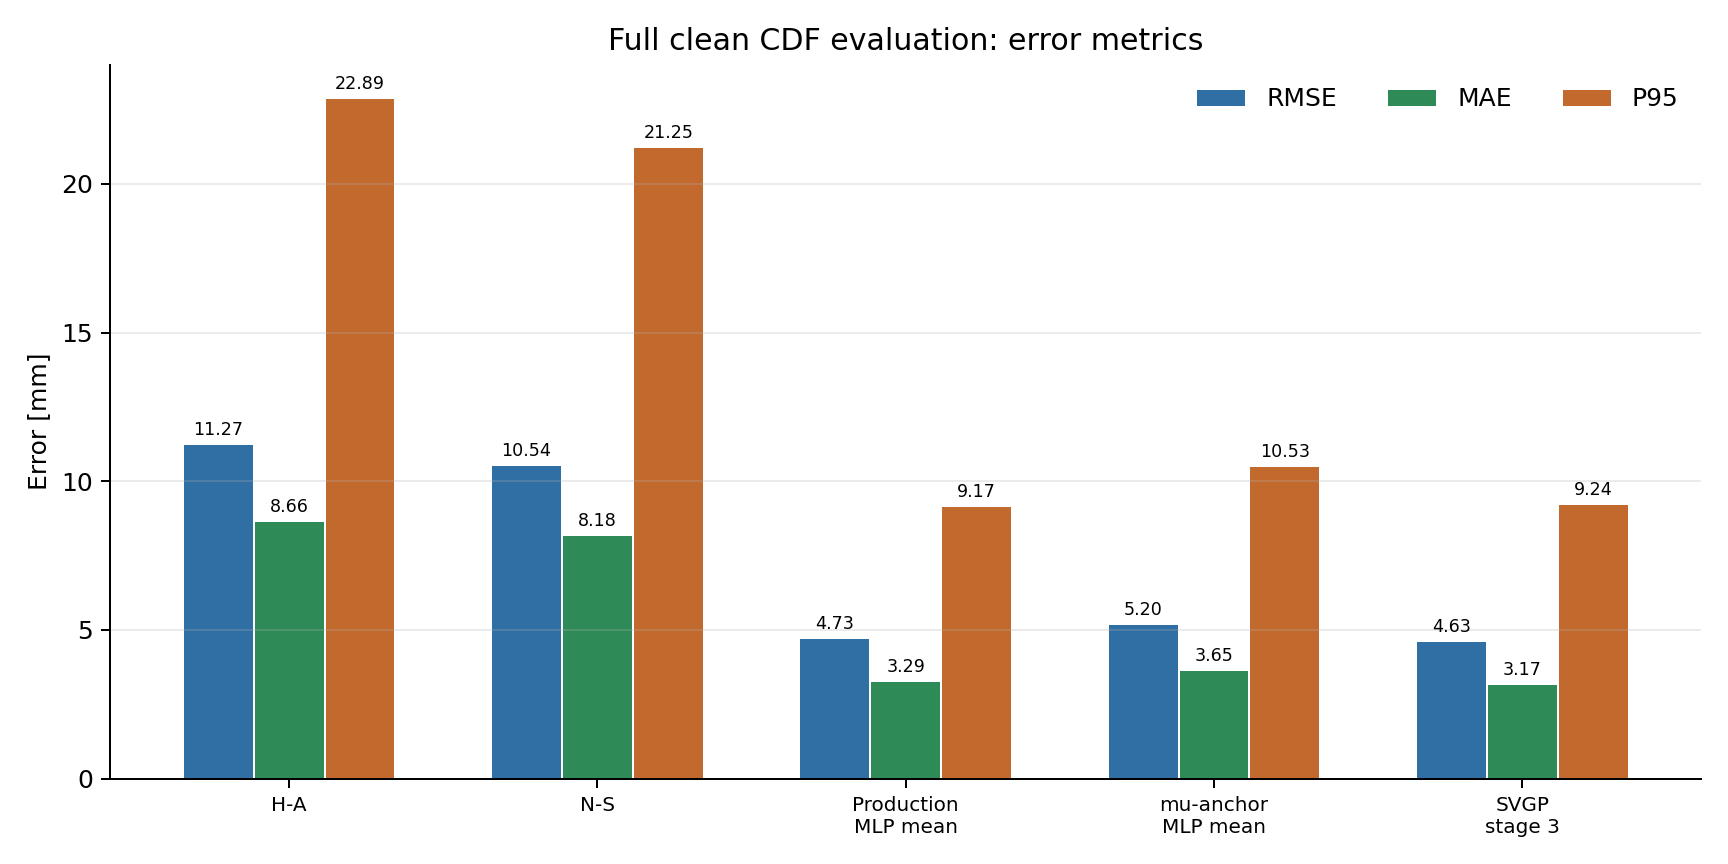
\includegraphics[width=0.86\linewidth]{images/baseline_comparison_20260521/full_clean_metric_bars_rmse_mae_p95.png}
\caption{full-clean CDF 协议下，生产 MLP 与物理基线、SVGP 替代主干在 RMSE、MAE 和尾部误差上的对比。}
\label{fig:metric-bars-current}
\end{figure}

同一组拟合后的 HA/NS 物理基线也重新在保守的未删失 CDF 点表上计算（数据归档路径详见附录~\ref{app:implementation_mapping}）。在这个 542{,}565 点子集上，生产 MLP 的 RMSE 为 \SI{4.265}{mm}，SVGP 的 RMSE 为 \SI{4.193}{mm}，两条物理曲线拟合基线仍远高于此：Hiroyasu--Arai 为 \SI{10.261}{mm}，Naber--Siebers 为 \SI{9.286}{mm}。在同一协议下，生产 MLP 的 1$\sigma$/2$\sigma$ 覆盖率为 0.887/0.989，而 SVGP 为 0.716/0.945，这证实了 MLP 的补偿优势是保守覆盖而非更低的点误差。在五次重复生产训练中，全净化 RMSE 标准差为 \SI{0.037}{mm}，范围在 \SIrange{4.689}{4.768}{mm} 之间；在未删失 CDF 点表上的标准差为 \SI{0.040}{mm}，范围在 \SIrange{4.217}{4.310}{mm} 之间。这一极窄的范围表明，尽管在当前固定表对比中 SVGP 仍是最强点预测器，生产结果并非种子随机的偶然。

\subsection{P50/Q1 工况级检查}

在逐点 CDF 指标之外，另外两个协议进一步锐化了 SVGP 与 MLP 的对比。在包含 4{,}213 个点的工况级 P50 集合上，直接拟合 P50 观测的 oracle q1 达到了 \SI{1.010}{mm} 的 RMSE 下限（不可部署）；在学习模型中，SVGP 领先（RMSE \SI{2.649}{mm}），生产 MLP 紧随其后（\(\SI{2.848}{mm}\pm\SI{0.059}{mm}\)），而面向外推正则化的诊断 KD 变体表现最差（\(\SI{3.212}{mm}\pm\SI{0.245}{mm}\)）。然而，在观测到的 P50 窗口之外包含 21{,}527 个点的 q1 外推网格上，排序发生了反转：诊断 KD 变体取得了最低的 RMSE（\(\SI{10.358}{mm}\pm\SI{0.106}{mm}\)）和最小的正向外推偏差（\SI{+6.269}{mm}），领先于 SVGP（\SI{10.591}{mm}，偏差 \SI{+6.410}{mm}）和生产 MLP（\(\SI{10.864}{mm}\pm\SI{0.064}{mm}\)，偏差 \SI{+6.753}{mm}）。这两种 MLP 变体因此探究了一个真正的权衡：生产无锚点模型是一个保守的分布内代理模型，而诊断 KD 变体被保留为一种受外推正则化的版本，在观测窗口外更接近 SVGP 风格的平滑先验。逐种子的详细数值及运行路径见附录~\ref{app:implementation_mapping}。

\begin{figure}[t]
\centering
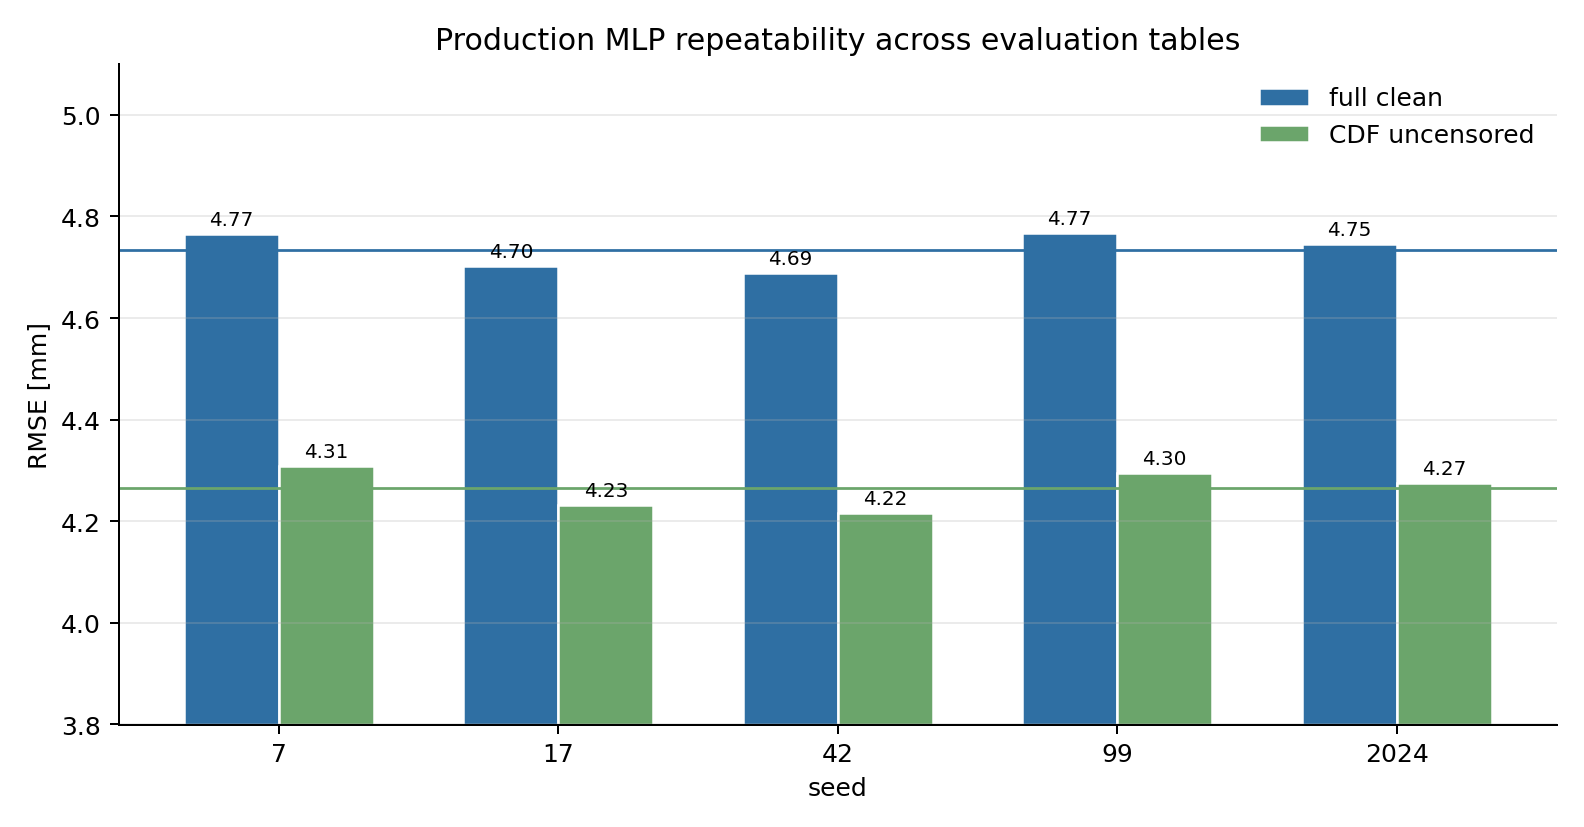
\includegraphics[width=0.80\linewidth]{images/baseline_comparison_20260521/production_mlp_per_seed_rmse.png}
\caption{五次重复生产训练（seeds 7/17/42/99/2024）的逐种子 RMSE，同时展示在 full-clean CDF 协议和保守 uncensored CDF 表上的结果。实线表示对应的五次运行均值。}
\label{fig:five-seed-rmse-current}
\end{figure}

为了展示误差结构，图~\ref{fig:latest-pred-residual} 使用最佳单次重复训练作为代表性诊断。散点整体沿恒等线分布，残差均值接近零，但高穿深区和困难喷嘴族仍存在更宽的误差尾部。谨慎的解读是，模型在其支持的域内已具备稳定的毫米级预测能力，但它并不是无条件外推器。

\begin{figure}[t]
\centering
\begin{minipage}{0.49\linewidth}
\centering
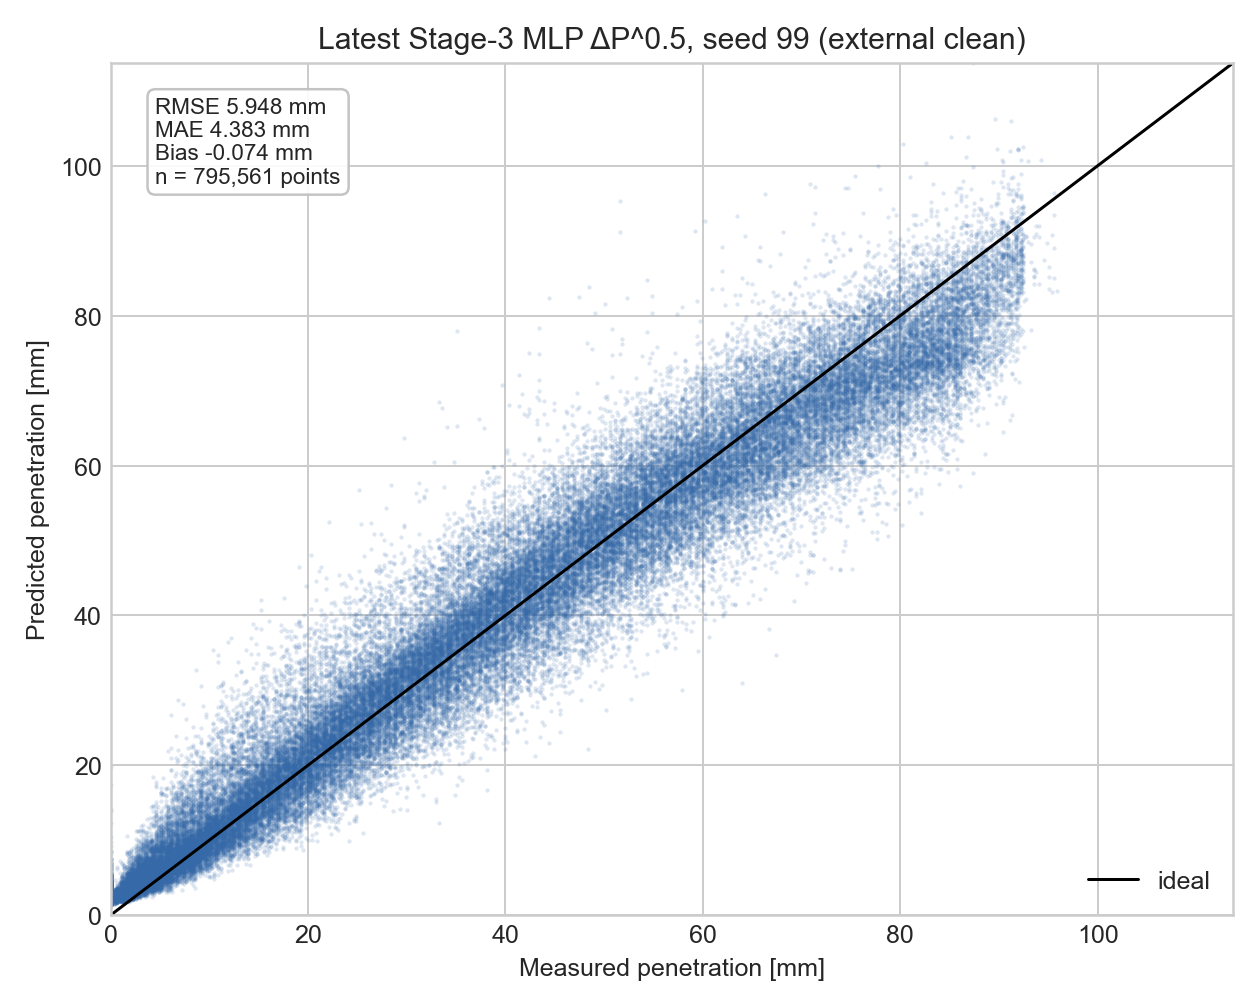
\includegraphics[width=\linewidth]{images/neural_network_fit_results/latest_pred_vs_actual_seed99.png}
\end{minipage}
\hfill
\begin{minipage}{0.49\linewidth}
\centering
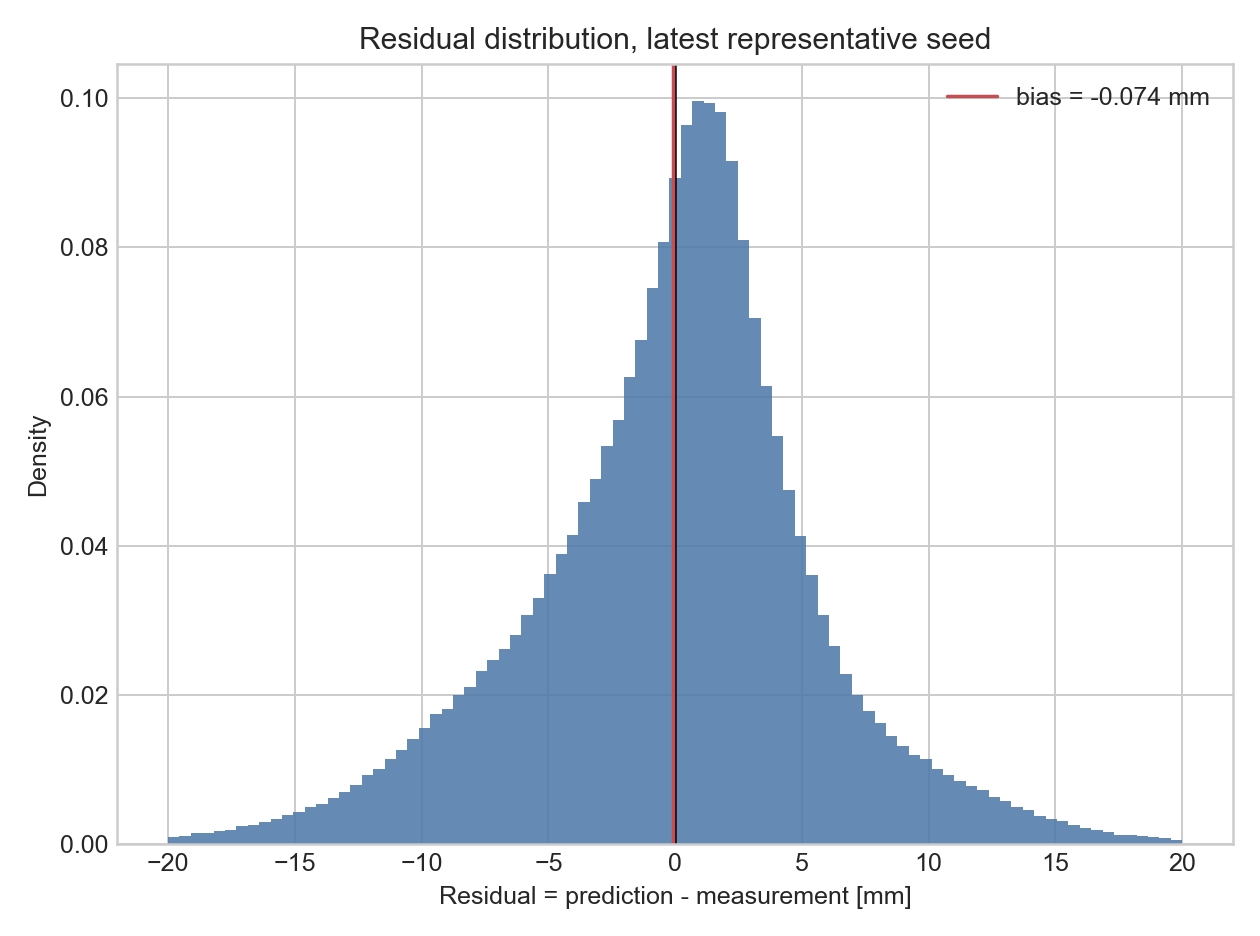
\includegraphics[width=\linewidth]{images/neural_network_fit_results/latest_residual_histogram_seed99.png}
\end{minipage}
\caption{代表性重复运行的预测与测量散点图和残差分布。此图用于诊断误差结构；核心对比使用上文刷新的五次生产运行均值。}
\label{fig:latest-pred-residual}
\end{figure}

\subsection{概率校准}

覆盖率检查只能测试少数几个置信区间，因此本文进一步使用可靠性图、连续排序概率分数（CRPS）和概率积分变换直方图。五种子生产 anchor-off 运行保持了显著低于物理基线的 CRPS，并且这种增益并非仅来自扩大不确定度区间：它来自均值精度与不确定度宽度之间更好的联合权衡。

图~\ref{fig:calibration-current} 展示了在同一 full-clean 诊断协议中加入 Stage~3 SVGP 后的可靠性图与 CRPS--sharpness 平面。三阶段 MLP（anchor-off）的 1$\sigma$/2$\sigma$ 覆盖率（五种子均值 0.867/0.985）高于名义高斯值，因此在外部清洗集合上是有意保守的。表~\ref{tab:external-clean-headline} 中刷新后的 Stage~3 对比显示，SVGP 现在是最强的点预测器（RMSE \SI{4.628}{mm}，1$\sigma$/2$\sigma$ 覆盖率 0.703/0.939），并在刷新后的校准诊断中获得了最低的 CRPS；而生产 MLP 仍是更为保守的筛查代理模型（RMSE \SI{4.735}{mm}，覆盖率远高于名义值）。因此，这两个模型应被理解为不同的精度--覆盖率权衡，而非单赢结果：SVGP 更接近名义覆盖率，而 MLP 为下游筛查保留了更宽的不确定度裕度。

\begin{figure}[t]
\centering
\begin{minipage}{0.49\linewidth}
\centering

\includegraphics[width=\linewidth]{images/calibration_20260521/reliability_overlay.png}
\end{minipage}
\hfill
\begin{minipage}{0.49\linewidth}
\centering

\includegraphics[width=\linewidth]{images/calibration_20260521/crps_sharpness_scatter.png}
\end{minipage}
\caption{概率预测诊断。左：可靠性图。右：连续排序概率分数与平均预测标准差的关系。对比包含物理基线、五个生产 MLP 种子及 Stage~3 SVGP 替代主干。}
\label{fig:calibration-current}
\end{figure}

\subsection{LONO 转移与 OOD 失效}

留一喷嘴族评估用于检查模型是否仅仅在训练期间已见的喷嘴族内插值。在锁定阶段二教师为仅 $\mu$-锚点配置并采用刷新后的五折 LONO 协议（留出喷嘴族 Nozzle0、Nozzle1、Nozzle2、Nozzle4、Nozzle5）下，LONO 胜出的阶段三 MLP 变体（不确定区间混合原始/KD 监督）的五折平均 RMSE 为 \(\SI{12.55}{mm}\pm\SI{12.46}{mm}\)，MAE 为 \(\SI{9.80}{mm}\pm\SI{10.18}{mm}\)，平均 1$\sigma$/2$\sigma$ 覆盖率为 0.575/0.770。同一未删失 LONO 评估测得阶段三 SVGP 的 RMSE 为 \(\SI{10.16}{mm}\pm\SI{9.57}{mm}\)，MAE 为 \(\SI{7.87}{mm}\pm\SI{7.55}{mm}\)，覆盖率为 0.628/0.821。跨喷嘴族的结论因此是有条件的：SVGP 是点转移更强的主干，而 MLP 的保留依据是其域内的保守覆盖、喷射起始辅助输出以及消融可负担性（按 §4 开头的术语约定理解）。

极高的标准差主要由 Nozzle0 这一折驱动，它是整个 campaign 中唯一的初代喷嘴几何。Nozzle0 最好被理解为一个跨设计族失效的外推案例，而非普通的平均性能折：阶段三 MLP 在此折的 RMSE 达到 \SI{34.76}{mm}，SVGP 的 RMSE 达到 \SI{26.99}{mm}，二者均存在系统性低估。如果排除 Nozzle0，MLP 的四折平均 RMSE 降至 \(\SI{7.00}{mm}\pm\SI{1.18}{mm}\)，而 SVGP 达到 \(\SI{5.95}{mm}\pm\SI{1.98}{mm}\)。此时覆盖率的对比交错：1$\sigma$ 覆盖率几乎相同（MLP 0.696 对 SVGP 0.697），而 MLP 的 2$\sigma$ 覆盖率更高（0.923 对 0.890）。因此 LONO 证据反驳了 MLP 全面占优的主张，转而把域内保守部署与跨喷嘴族转移精度分开评估。

\begin{figure}[t]
\centering
\begin{minipage}{0.49\linewidth}
\centering
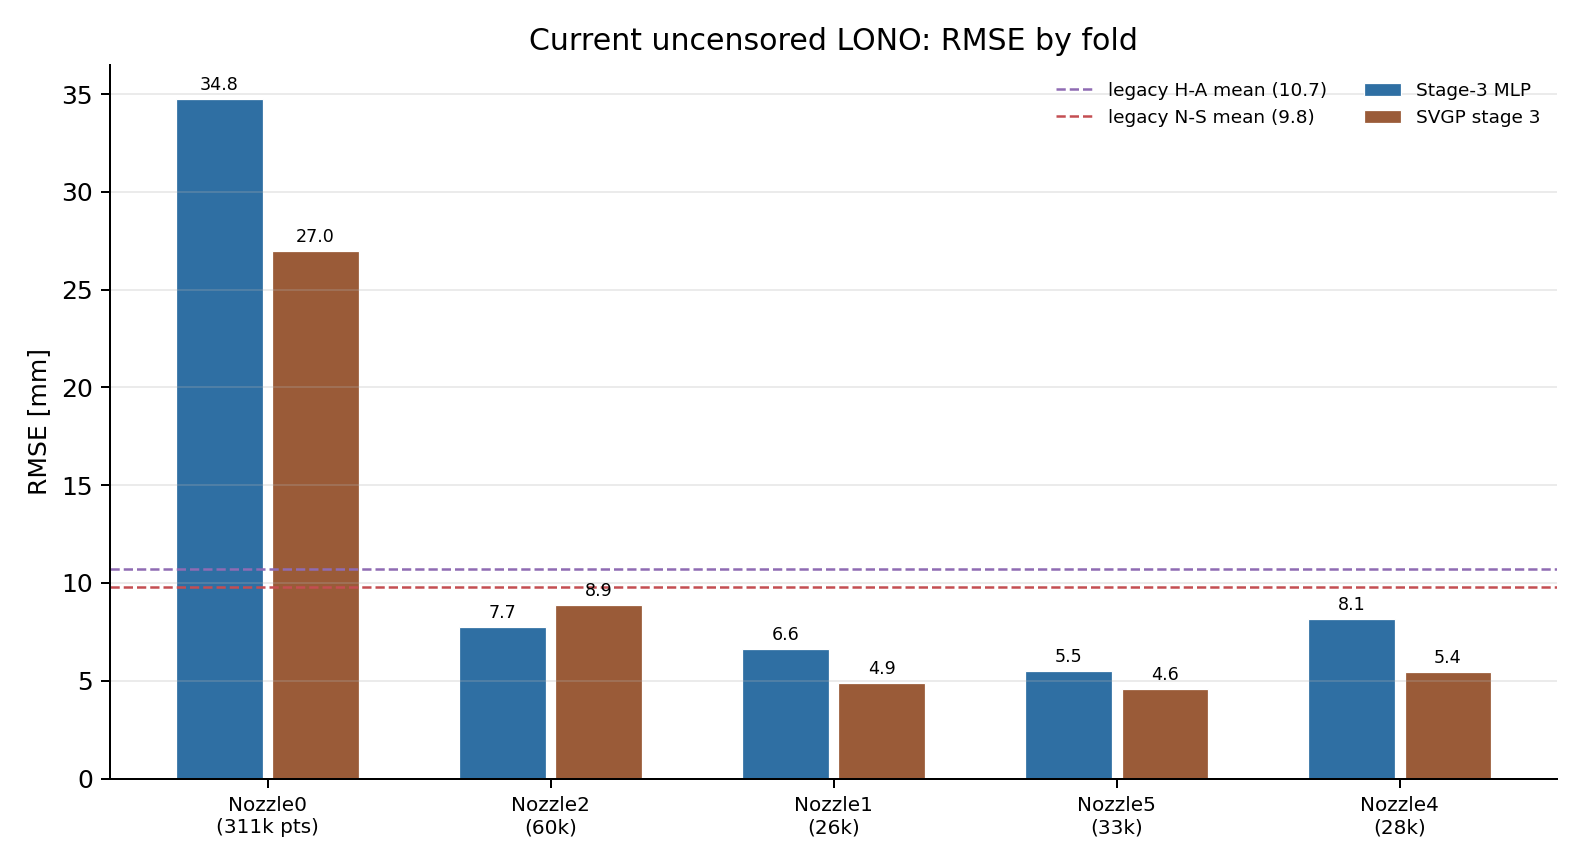
\includegraphics[width=\linewidth]{images/lono_20260509/lono_rmse_by_fold.png}
\end{minipage}
\hfill
\begin{minipage}{0.49\linewidth}
\centering
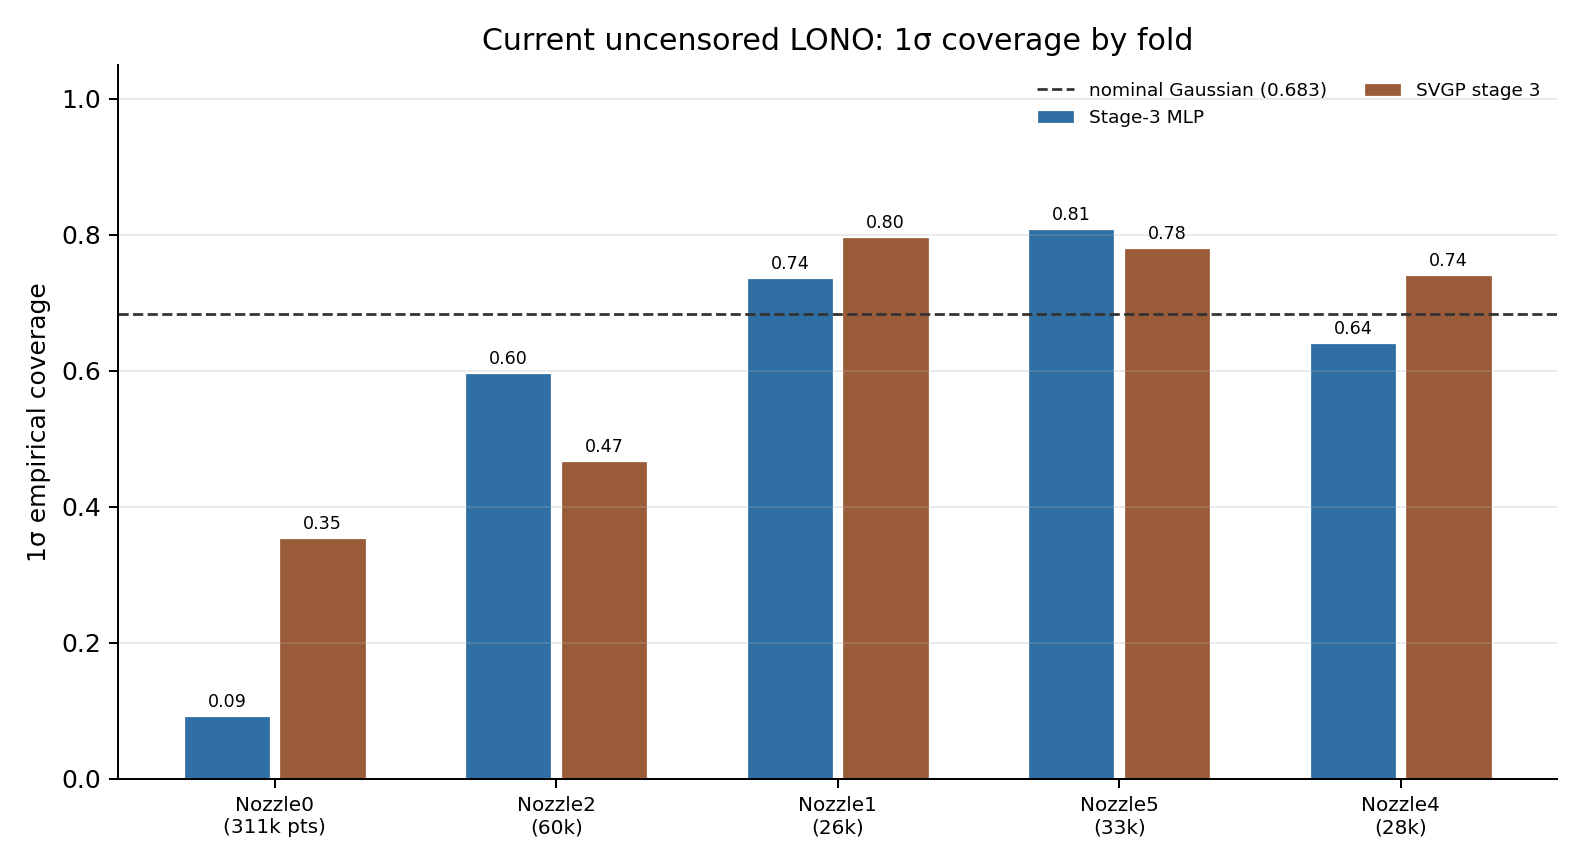
\includegraphics[width=\linewidth]{images/lono_20260509/lono_coverage_by_fold.png}
\end{minipage}
\caption{当前未删失 LONO 跨架构诊断。左：阶段三 MLP LONO 胜出变体与阶段三 SVGP 的各折 RMSE；传统 HA/NS LONO RMSE 均值仅作为虚线尺度参考。右：相同未删失协议下的各折 1$\sigma$ 覆盖率，虚线表示名义高斯水平。}
\label{fig:lono-current}
\end{figure}

\subsubsection{针对 SVGP 替代主干的跨架构 LONO 对比}
\label{sec:svgp-lono-comparison-zh}

为测试同样的删失感知回归协议在不同模型家族中的表现，本文在相同的五折 LONO 划分下，使用稀疏异方差高斯过程（SVGP）替代主干（阶段三模式）重新运行，其在拼接了原始 CDF 点观测的合成目标上进行训练，以匹配阶段三 MLP 的监督机制。在保存的模型工件允许范围内，所有其他轴（五个留出喷嘴族、生产输入特征集、训练后未删失评估脚本）均保持固定。物理 LONO 行仅作为遗留 RMSE 的刻度参考保留，因为在当前归档中，这些基线缺少同协议下的 MAE 和覆盖率表。

\begin{table}[t]
\centering
\footnotesize
\begin{tabular}{@{}L{0.34\linewidth}rrrr@{}}
\toprule
模型 & RMSE [mm] & MAE [mm] & 1$\sigma$ 覆盖率 & 2$\sigma$ 覆盖率 \\
\midrule
校准后的 Hiroyasu--Arai，遗留 LONO 参考 & 10.713 \(\pm\) 1.542 & --- & --- & --- \\
带延迟项的 Naber--Siebers，遗留 LONO 参考 & 9.784 \(\pm\) 2.102 & --- & --- & --- \\
三阶段 MLP，阶段三 LONO 胜出变体 & 12.55 \(\pm\) 12.46 & 9.80 \(\pm\) 10.18 & 0.575 & 0.770 \\
稀疏异方差 GP，阶段三模式 & \textbf{10.16 \(\pm\) 9.57} & \textbf{7.87 \(\pm\) 7.55} & \textbf{0.628} & \textbf{0.821} \\
三阶段 MLP，排除 Nozzle0 & 7.00 \(\pm\) 1.18 & 5.25 \(\pm\) 0.81 & 0.696 & \textbf{0.923} \\
稀疏异方差 GP，排除 Nozzle0 & \textbf{5.95 \(\pm\) 1.98} & \textbf{4.55 \(\pm\) 1.55} & \textbf{0.697} & 0.890 \\
\bottomrule
\end{tabular}
\caption{跨架构 LONO 对比。MLP 和 SVGP 行报告了在五个留一喷嘴族折中使用当前未删失评估工件的未加权均值和标准差。破折号表示当前归档中无法追溯同协议下的 MAE 和覆盖率数据。粗体表示在该比较列中最优的阶段三架构。}
\label{tab:svgp-lono-comparison}
\end{table}

\begin{figure}[t]
\centering
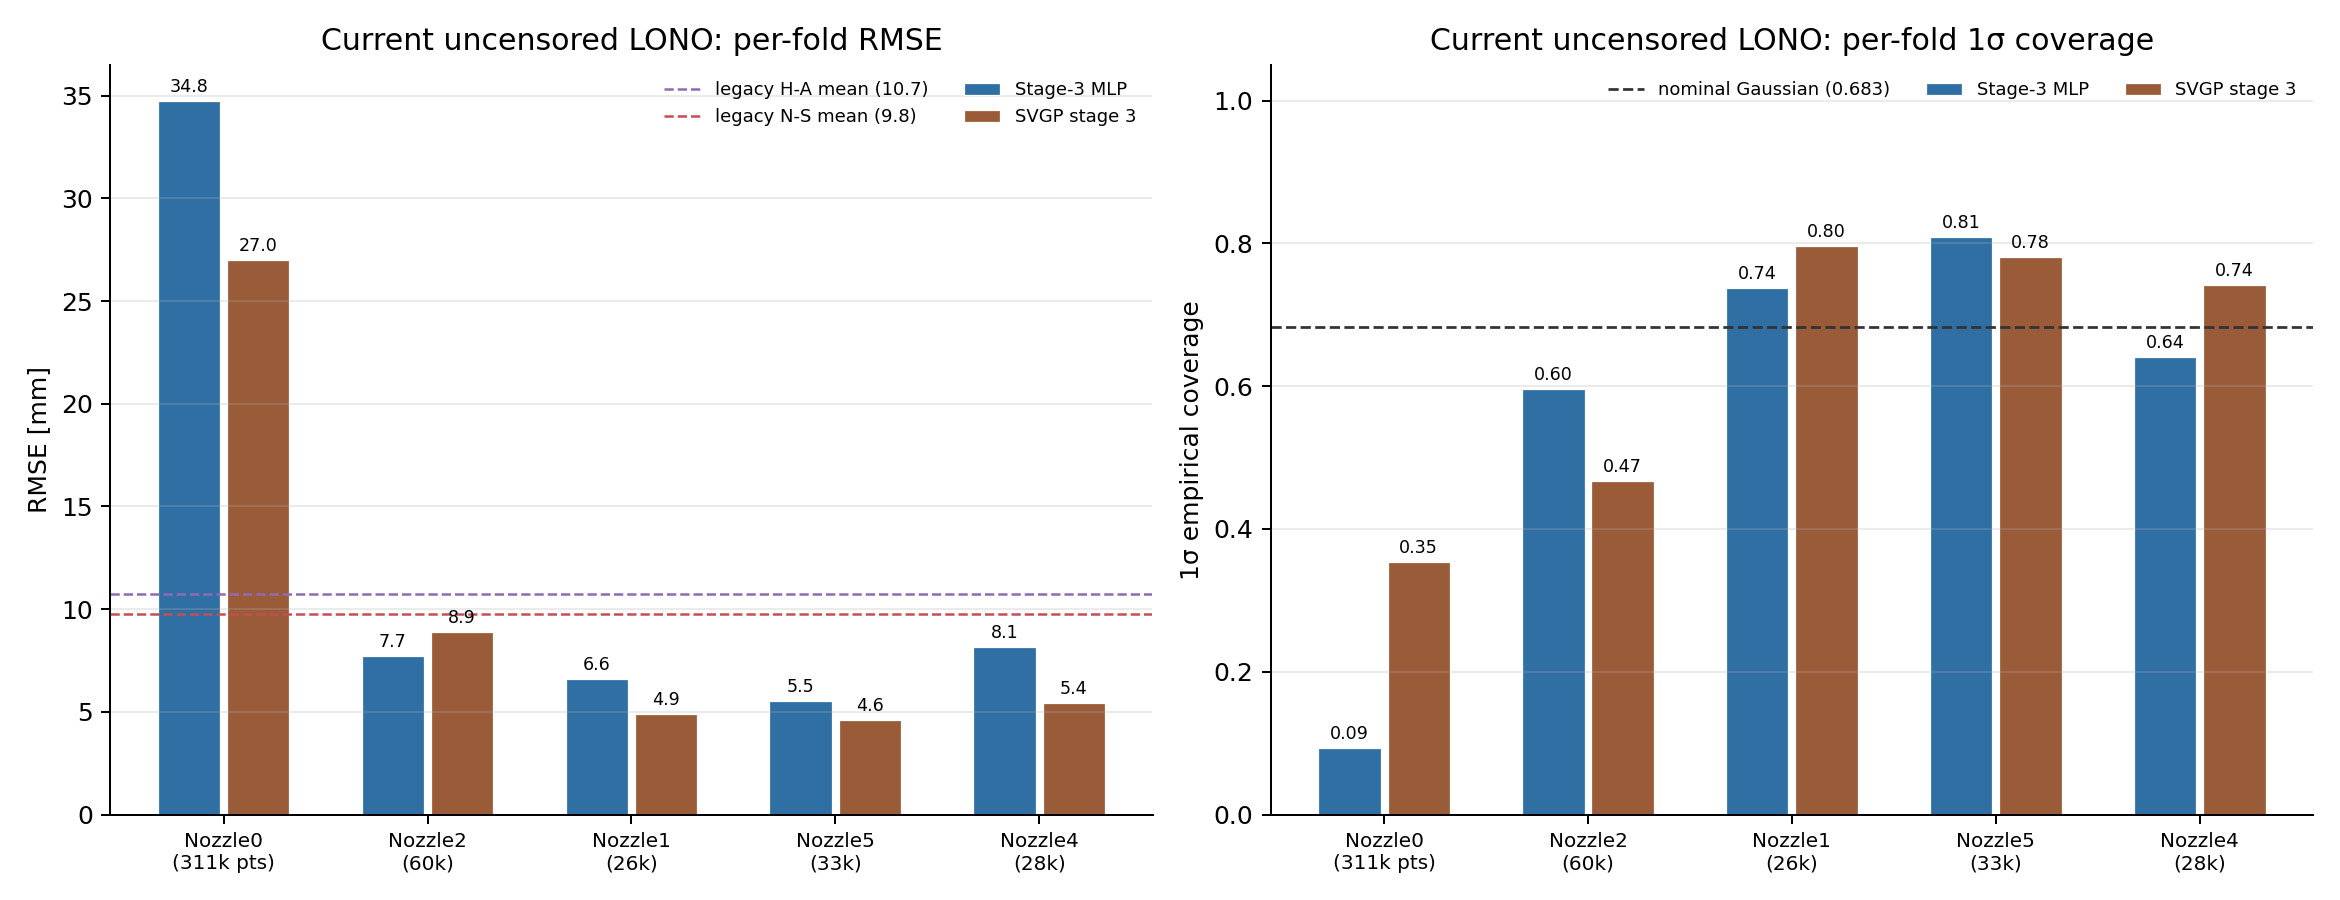
\includegraphics[width=\linewidth]{images/svgp_lono_comparison.png}
\caption{阶段三 MLP 与稀疏异方差 GP 在当前未删失 LONO 协议下的综合诊断。左图报告各留出喷嘴族的 RMSE；右图报告经验 1$\sigma$ 覆盖率，虚线为名义高斯水平。}
\label{fig:svgp-lono-comparison}
\end{figure}

正式的跨架构结论仅基于阶段三 MLP 和阶段三 SVGP 两行，因为只有这两行在同一未删失 LONO 协议下具备完整的当前评估工件。结果明确：无论是否包含 Nozzle0，核主干都取得了更低的 RMSE 和 MAE。MLP 剩下的优势不在于 OOD 上的点预测精度，而在于围绕这个低维代理模型的更广泛工作流——喷射起始辅助预测头、区制感知 KD、域内保守覆盖，以及下文记录的低开销消融网格。

\subsubsection{方法论说明：双协议评估}
\label{sec:dual-protocol-zh}

本章使用的两种评估协议——上文报告的 LONO 交叉验证以及后文第~\ref{sec:kd-form-fix-zh} 节报告的五种子生产 bootstrap——是有意区别开的，回答的是不同问题。LONO 协议在训练时整族留出一个喷嘴族，测量模型对训练中从未见过的喷嘴几何的泛化能力，因此报告的是模型的\textbf{域外（OOD）}行为。生产协议在全数据集上使用五个随机种子重新训练同一配置，并在非右删失测试集上评估；它测量的是模型的\textbf{域内拟合质量}及其对随机初始化的敏感性，是核心表中方差报告的合适协议。

这两个协议并列报告而不合并为单一排名，因为各自隔离了独立的论断。一个在 LONO 协议下胜出但在生产 bootstrap 下落败的模型，意味着泛化好但域内拟合差；反之，在生产 bootstrap 胜出但 LONO 落败的模型，意味着域内拟合紧密但对外推至新喷嘴几何的表现差。生产协议支持 MLP 作为测量设计空间内的保守筛查代理；LONO 协议则表明 SVGP 替代主干在跨喷嘴族转移的点精度上更强。这些是互补的论断，而不是对某一架构的全面胜利宣告。

\subsubsection{各 campaign 文件夹间的差异与代表性轨迹案例}

误差在不同 campaign 文件夹之间并不均匀。图~\ref{fig:per-folder-rmse-best} 展示了最终模型在各评估子文件夹上的单条轨迹 RMSE 均值与中位数。最容易的文件夹仍处于低 \SI{3}{mm} 区间，而最困难的接近 \SI{9}{mm}。Nozzle0 处于这个排序的中间而不是两端，因此最终消融带来的全局改善并不是由某一个匿名化参考 campaign 单独驱动的。

代表性案例使这种差异更直观。图~\ref{fig:traj-best-case} 给出一个表现最好的案例，其中预测均值紧密跟随测量 plume 轨迹，且不确定度带相对较窄。图~\ref{fig:traj-worst-case} 给出了一个困难的案例，模型依然保持单调且不确定度带适当变宽，但若干 plume 仍表现出系统性的形状失配或延迟上升。这个困难案例并不包含删失轨迹，因此残余误差不能完全归因于视场丢失；依赖喷嘴族的早期瞬态依然是真正的建模难点。

\begin{figure}[t]
\centering
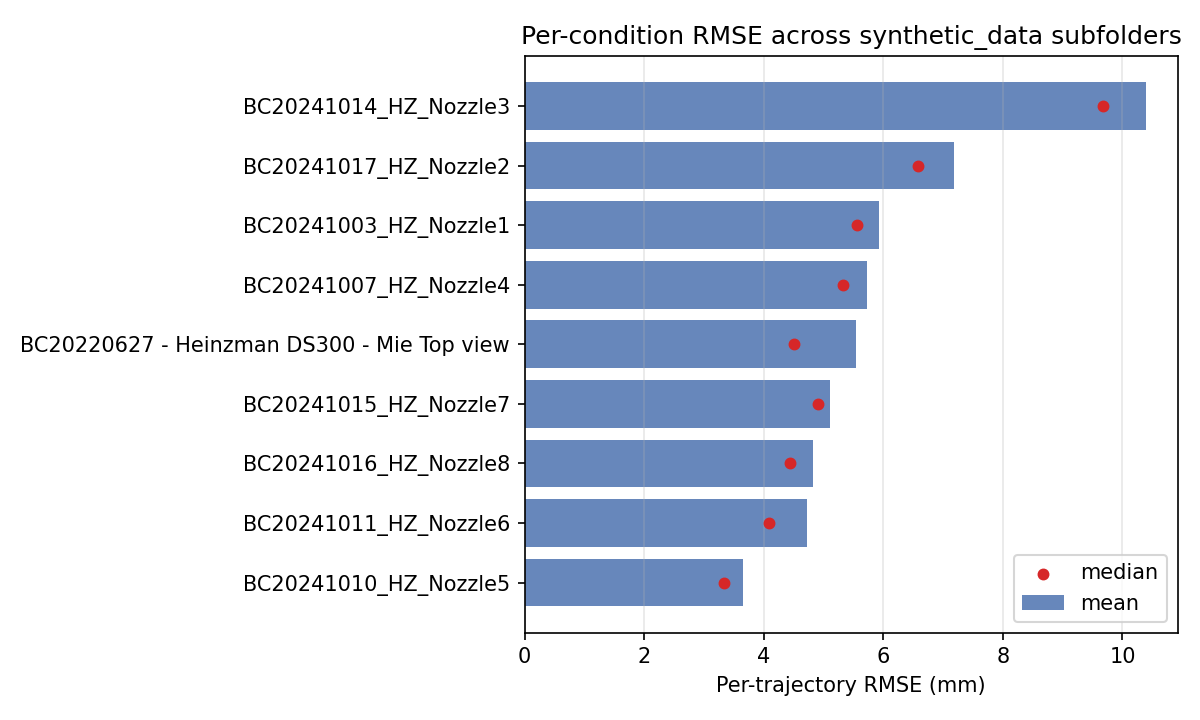
\includegraphics[width=0.88\linewidth]{images/neural_network_fit_results/per_folder_rmse_best.png}
\caption{最终 Stage~3 模型在各评估 campaign 文件夹上的单条轨迹 RMSE 均值与中位数。}
\label{fig:per-folder-rmse-best}
\end{figure}

\begin{figure}[p]
\centering
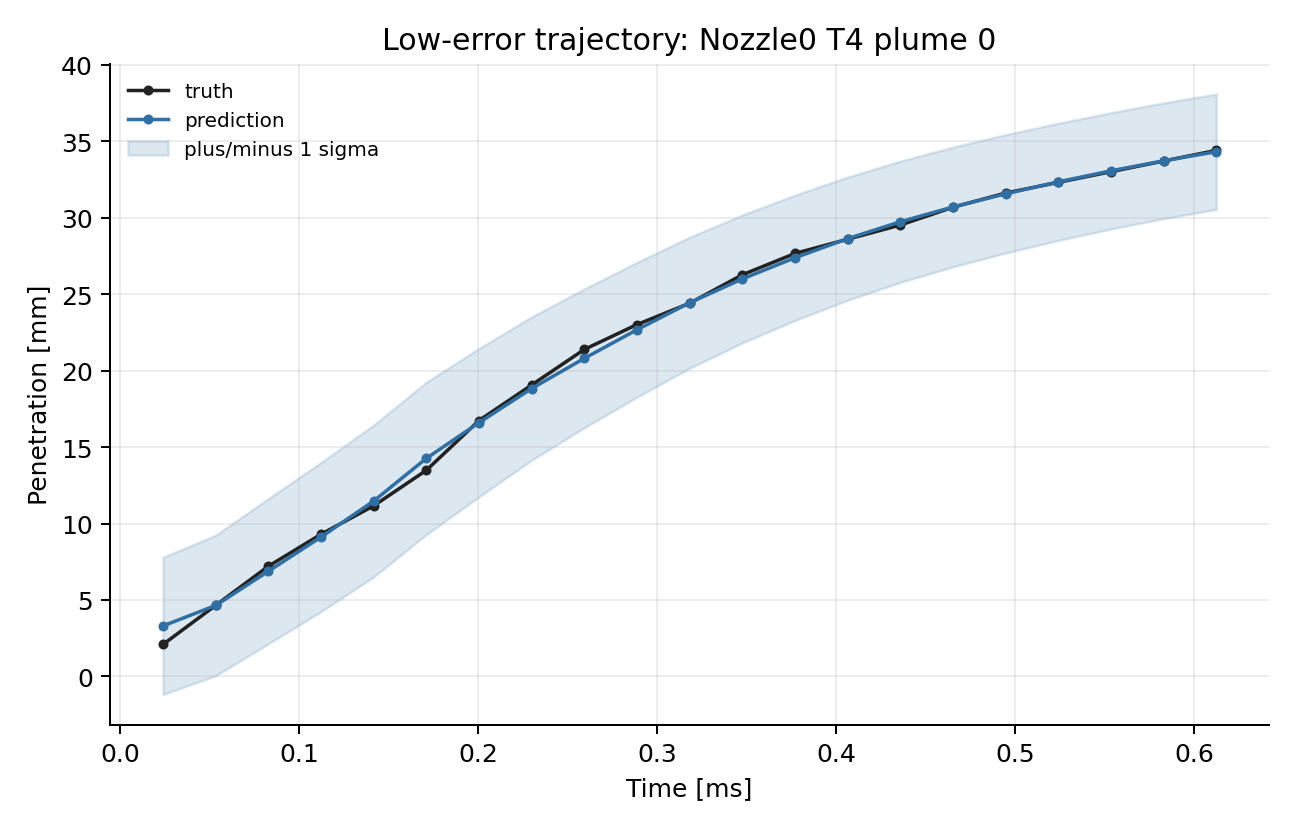
\includegraphics[width=\linewidth]{images/neural_network_fit_results/traj_best_nozzle7_T19.png}
\caption{最终 Stage~3 模型的代表性最佳案例。预测均值紧密跟随测量 plume 轨迹，且在所展示的 plume 上不确定度带保持较窄。}
\label{fig:traj-best-case}
\end{figure}

\begin{figure}[p]
\centering
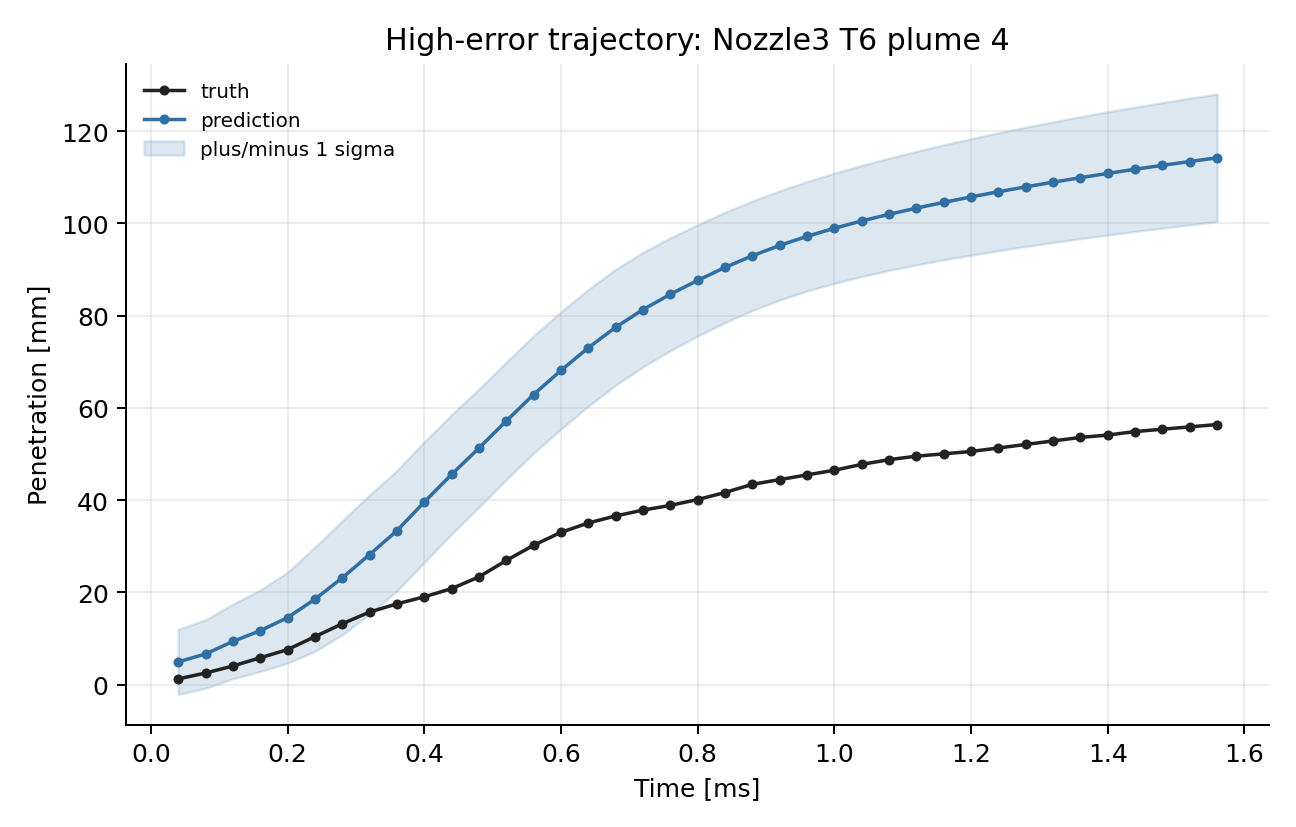
\includegraphics[width=\linewidth]{images/neural_network_fit_results/traj_worst_nozzle3_T3.png}
\caption{最终 Stage~3 模型的代表性困难案例。模型依然保持单调且保守，但若干 plume 显示出系统性的形状失配，从而拉大了误差。}
\label{fig:traj-worst-case}
\end{figure}

\subsubsection{困难工况的视觉证据与失效模式剖析：以 Nozzle 3 为例}

留一喷嘴族（LONO）评估显示，代理模型在诸如 Nozzle~3 等特定喷嘴族上出现了覆盖率下降与误差放大。为观察这些困难工况在原始数据中的形态，本文将 Phantom 高速 Mie 散射图像与对应的逐喷油束穿深曲线进行了交叉比对（图~\ref{fig:failure-mode-nozzle3}）。

图像序列（$t \approx 0.6 \sim 1.0\,\si{ms}$）显示出明显的孔间非对称性：当左侧喷油束已建立稳定的连续射流时，右下方的三束喷油（约 3 至 5 点钟方向）却显得短小、断续。其中部分喷孔先挤出少量低动量、脱离主体的先导液团，并在环境气阻下迅速减速；这一视觉观察对应于穿深曲线（如 Plume~2 的绿线、Plume~0 的蓝线）在同一时间窗内出现的``平顶''特征。随后（$t > 1.0\,\si{ms}$），在同一方位出现了主射流并迅速反超先导液团，使曲线呈现阶跃式陡升。

这种``先导液团 + 反超主射流''的轨迹形态，与分段或多段喷射文献中报道的尾迹驱动追赶/反超机制一致：先到达的液团可通过尾迹效应和轴向气动量预处理改变其后液团的穿深。因为本实验既无同步气速测量，也无内部流动可视化或液团身份追踪，该案例只能被解释为与此类机制``相一致的''图像证据；针阀偏摆或瞬态喷孔节流等机械原因同样是现有数据所不能排除的候选解释。

数据所能直接支持的，是建模层面的推论。降阶拟合目标（$k_{1/4}t^{1/4}$）按构造单调且呈凹形，无法包络这类二阶导数发生突变的阶跃轨迹。将平滑单调先验强加于这类轨迹会造成目标失真，这是导致 Stage~2、Stage~3 网络在受影响喷嘴族上覆盖率下降的一个可识别原因。要对此类极端瞬态喷雾进行建模，因此需要采用更柔性的形状先验，或者在能够分辨真实机制的诊断手段就位后，对该机制进行显式的条件化。

\begin{figure}[p]
\centering
\begin{minipage}{0.24\linewidth}
\centering
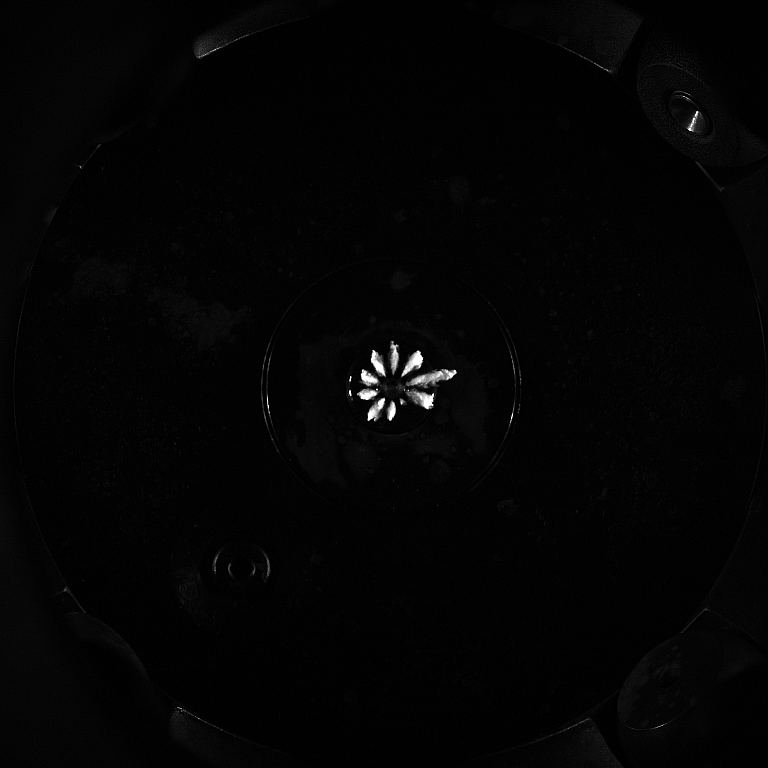
\includegraphics[width=\linewidth]{images/failure_mode_nozzle3/phantom_t3.png}\\
(a) $t\approx 0.6\sim0.8\,\si{ms}$
\end{minipage}
\hfill
\begin{minipage}{0.24\linewidth}
\centering
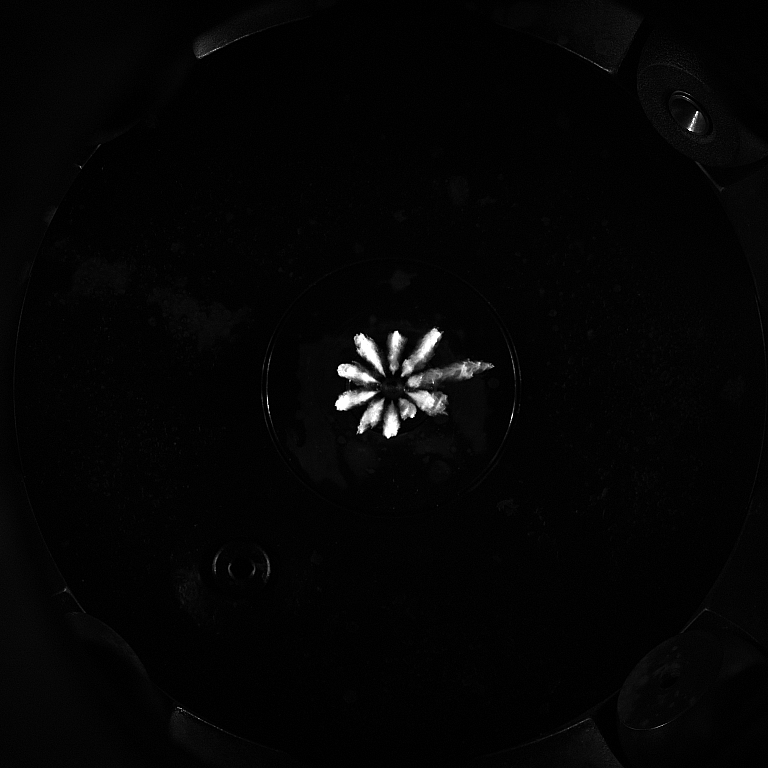
\includegraphics[width=\linewidth]{images/failure_mode_nozzle3/phantom_t4.png}\\
(b) $t\approx 0.8\,\si{ms}$
\end{minipage}
\hfill
\begin{minipage}{0.24\linewidth}
\centering
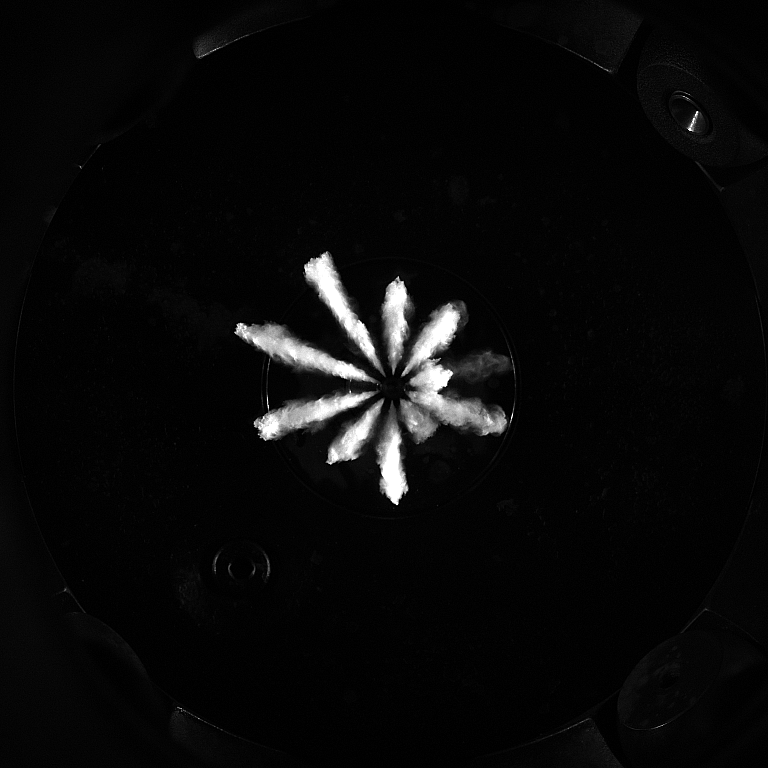
\includegraphics[width=\linewidth]{images/failure_mode_nozzle3/phantom_t5.png}\\
(c) $t\approx 1.0\,\si{ms}$
\end{minipage}
\hfill
\begin{minipage}{0.24\linewidth}
\centering
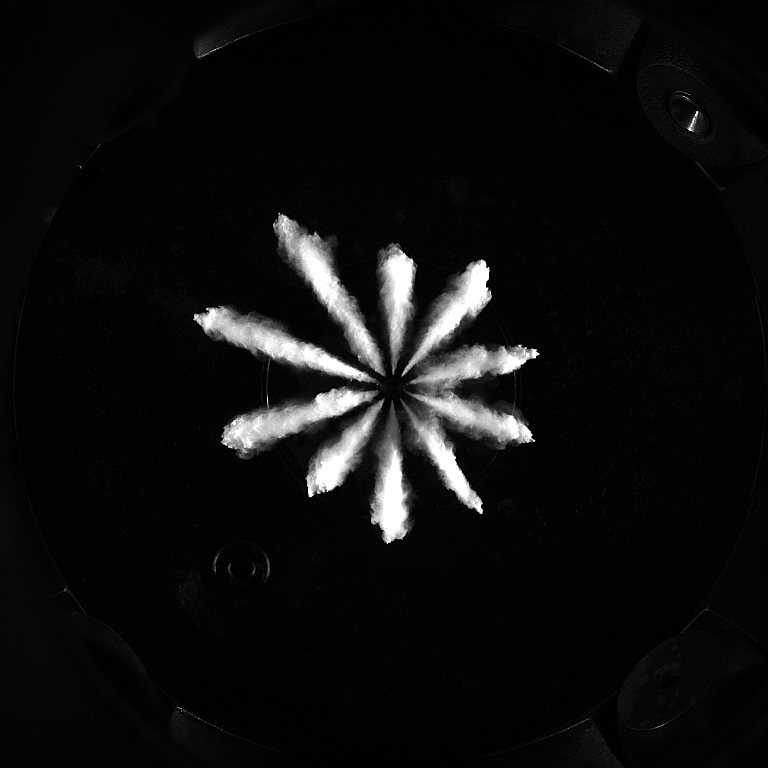
\includegraphics[width=\linewidth]{images/failure_mode_nozzle3/phantom_t6.png}\\
(d) $t > 1.0\,\si{ms}$
\end{minipage}

\vspace{1em}
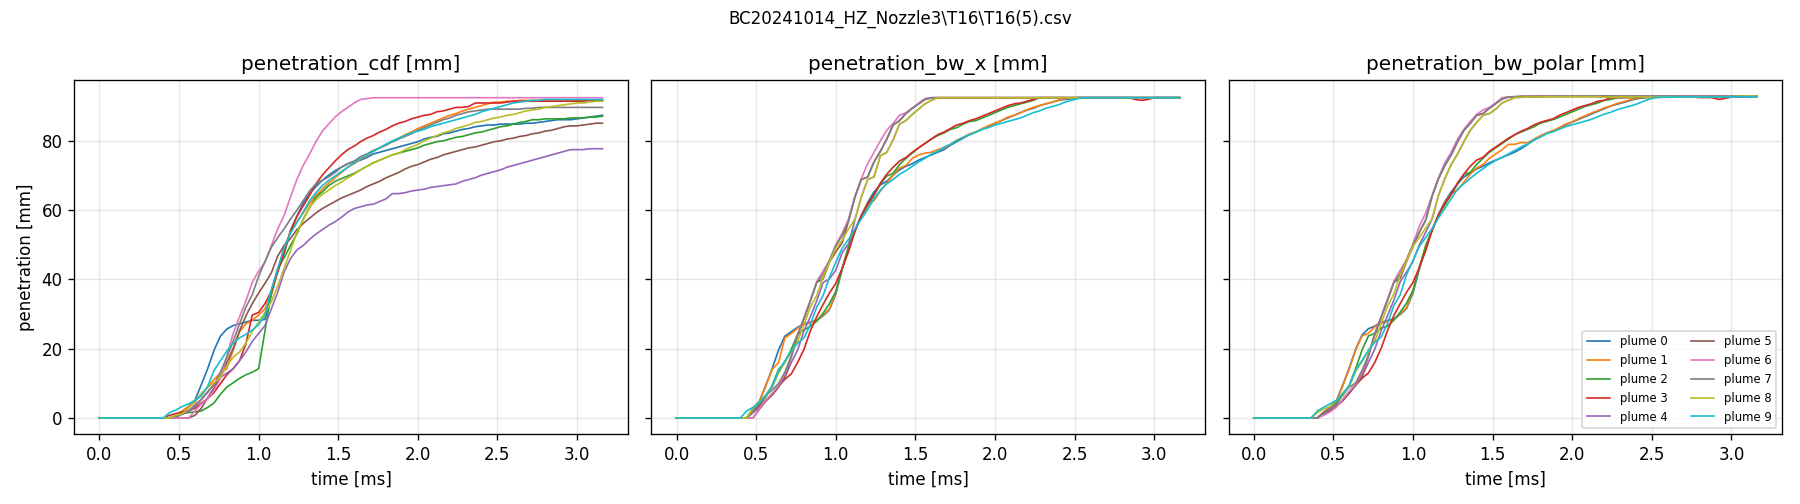
\includegraphics[width=0.95\linewidth]{images/failure_mode_nozzle3/nozzle3_t16_plot.png}
\caption{Nozzle 3 (T16 工况) 极端瞬态喷雾的视觉证据与对应穿深曲线。上排图像序列捕捉了右下方喷油束在初期受到严重节流并形成脱离先导液团，随后在 $t>1.0\,\si{ms}$ 爆发主射流的过程。下排穿深曲线中的 Plume 0（蓝线）和 Plume 2（绿线）精确反映了这一阶跃式轨迹，打破了代理模型平滑单调增长的数学假设。}
\label{fig:failure-mode-nozzle3}
\end{figure}

\subsection{MLP 消融证据与筛查演示}

前文章节确立了跨架构结果：SVGP 目前在点精度上是赢家（尤其在 LONO 转移协议下），而生产 MLP 则是域内更为保守的筛查代理模型。接下来的证据解释了为何 MLP 技术栈仍被保留作为运行工作流：它的训练课程可以被廉价地消融，其喷射起始辅助输出支持 GUI 原型，且它的区制感知蒸馏使得保守筛查行为具有可追溯性而非偶然。

\subsubsection{Stage-2 anchor 调度消融实验}
\label{sec:stage2-anchor-ablation-zh}

阶段二在异方差 NLL 之上引入了两个可选的早期 anchor 惩罚项：把 \(\mu(t{\to}0)\to 0\) 的二次惩罚（权重 \(\lambda_\mu\)）以及把超出固定下限 \(\sigma_{0}\) 的过多标准差 \(\max(0,\,\sigma(t{\to}0)-\sigma_{0})\) 拉小的二次惩罚（权重 \(\lambda_\sigma\)）。两者均与三角核 \(w(t)=\max(0,\,1-t/\tau)\) 加权积分，作用在 \(\tau=\SI{0.15}{ms}\) 的早期时间窗口。为检查这些 anchor 究竟是帮助还是损害跨喷嘴族泛化，本文在与阶段一相同的 LONO 协议下对比了三个阶段二变体：(i)~无 anchor（\(\lambda_\mu=\lambda_\sigma=0\)）；(ii)~仅 $\mu$-anchor（\(\lambda_\mu=10^{-2}\)，\(\lambda_\sigma=0\)）；(iii)~$\mu$+$\sigma$ 双 anchor（\(\lambda_\mu=10^{-2}\)，\(\lambda_\sigma=10^{-3}\)）。三个变体共用阶段一胜出的生产七特征配置（$\alpha=0.5$ 带压力残差）作为热启动，共用相同的五折 LONO 划分、相同的阶段三无锚点蒸馏链、相同的网络架构与优化器、以及单一固定种子（42）；唯一变化的轴是阶段二的 anchor 配置。本节中的留出集指标是在完整的阶段一$\to$二$\to$三流水线之后，基于留出喷嘴族的未截断 CDF~P50 点进行评估的（各折评估点数依次为：Nozzle0 311{,}149、Nozzle2 60{,}369、Nozzle5 33{,}017、Nozzle4 28{,}139、Nozzle1 25{,}705）。

\begin{table}[t]
\centering
\footnotesize
\setlength{\tabcolsep}{4pt}
\begin{tabular}{@{}L{0.30\linewidth}rrrr@{}}
\toprule
变体 & RMSE [mm] & MAE [mm] & Bias [mm] & 1$\sigma$ / 2$\sigma$ 覆盖率 \\
\midrule
\texttt{no\_anchor}        & 14.54 $\pm$ 12.36 & 10.80 $\pm$ \phantom{0}9.96 & $-8.50 \pm 11.03$ & 0.602 / 0.763 \\
\texttt{mu\_anchor}        & \textbf{12.73 $\pm$ 12.44} & \textbf{\phantom{0}9.86 $\pm$ 10.22} & \textbf{\boldmath$-7.11 \pm 11.51$} & 0.570 / \textbf{0.775} \\
\texttt{mu\_sigma\_anchor} & 13.05 $\pm$ 12.46 & 10.06 $\pm$ 10.33 & $-7.59 \pm 11.45$ & 0.564 / 0.764 \\
\bottomrule
\end{tabular}
\caption{阶段二 anchor 调度 LONO 消融实验。每一行是五折留一喷嘴族（Nozzle0、Nozzle1、Nozzle2、Nozzle4、Nozzle5）的留出集均值~$\pm$~标准差。最终选定的阶段二教师配置为仅 $\mu$-anchor（表中第二行），它在 RMSE、MAE、偏差幅度与 2$\sigma$ 覆盖率上同时胜出。}
\label{tab:stage2-anchor-ablation}
\end{table}

\begin{table}[t]
\centering
\footnotesize
\setlength{\tabcolsep}{4pt}
\begin{tabular}{@{}L{0.28\linewidth}rrrrr|r@{}}
\toprule
变体 & Nozzle0 & Nozzle1 & Nozzle2 & Nozzle4 & Nozzle5 & 均值 \\
\midrule
\texttt{no\_anchor}        & 34.25 & \phantom{0}6.56 & 19.18 & 7.57 & 5.11 & 14.54 \\
\texttt{mu\_anchor}        & 34.92 & \phantom{0}7.16 & \textbf{\phantom{0}7.76} & 8.20 & 5.60 & \textbf{12.73} \\
\texttt{mu\_sigma\_anchor} & 35.12 & \phantom{0}7.10 & 10.04 & 7.73 & 5.27 & 13.05 \\
\bottomrule
\end{tabular}
\caption{三种阶段二 anchor 变体的各折 LONO RMSE [mm]。三者都在 Nozzle0 折上失效（第一代喷嘴几何，真正的跨设计族外推；以点数占据主导位置）；真正起区分作用的是 Nozzle2 折，无 anchor 较仅 $\mu$-anchor 增加了 \SI{11.4}{mm} 的 RMSE。}
\label{tab:stage2-anchor-ablation-per-fold}
\end{table}

\begin{figure}[t]
\centering
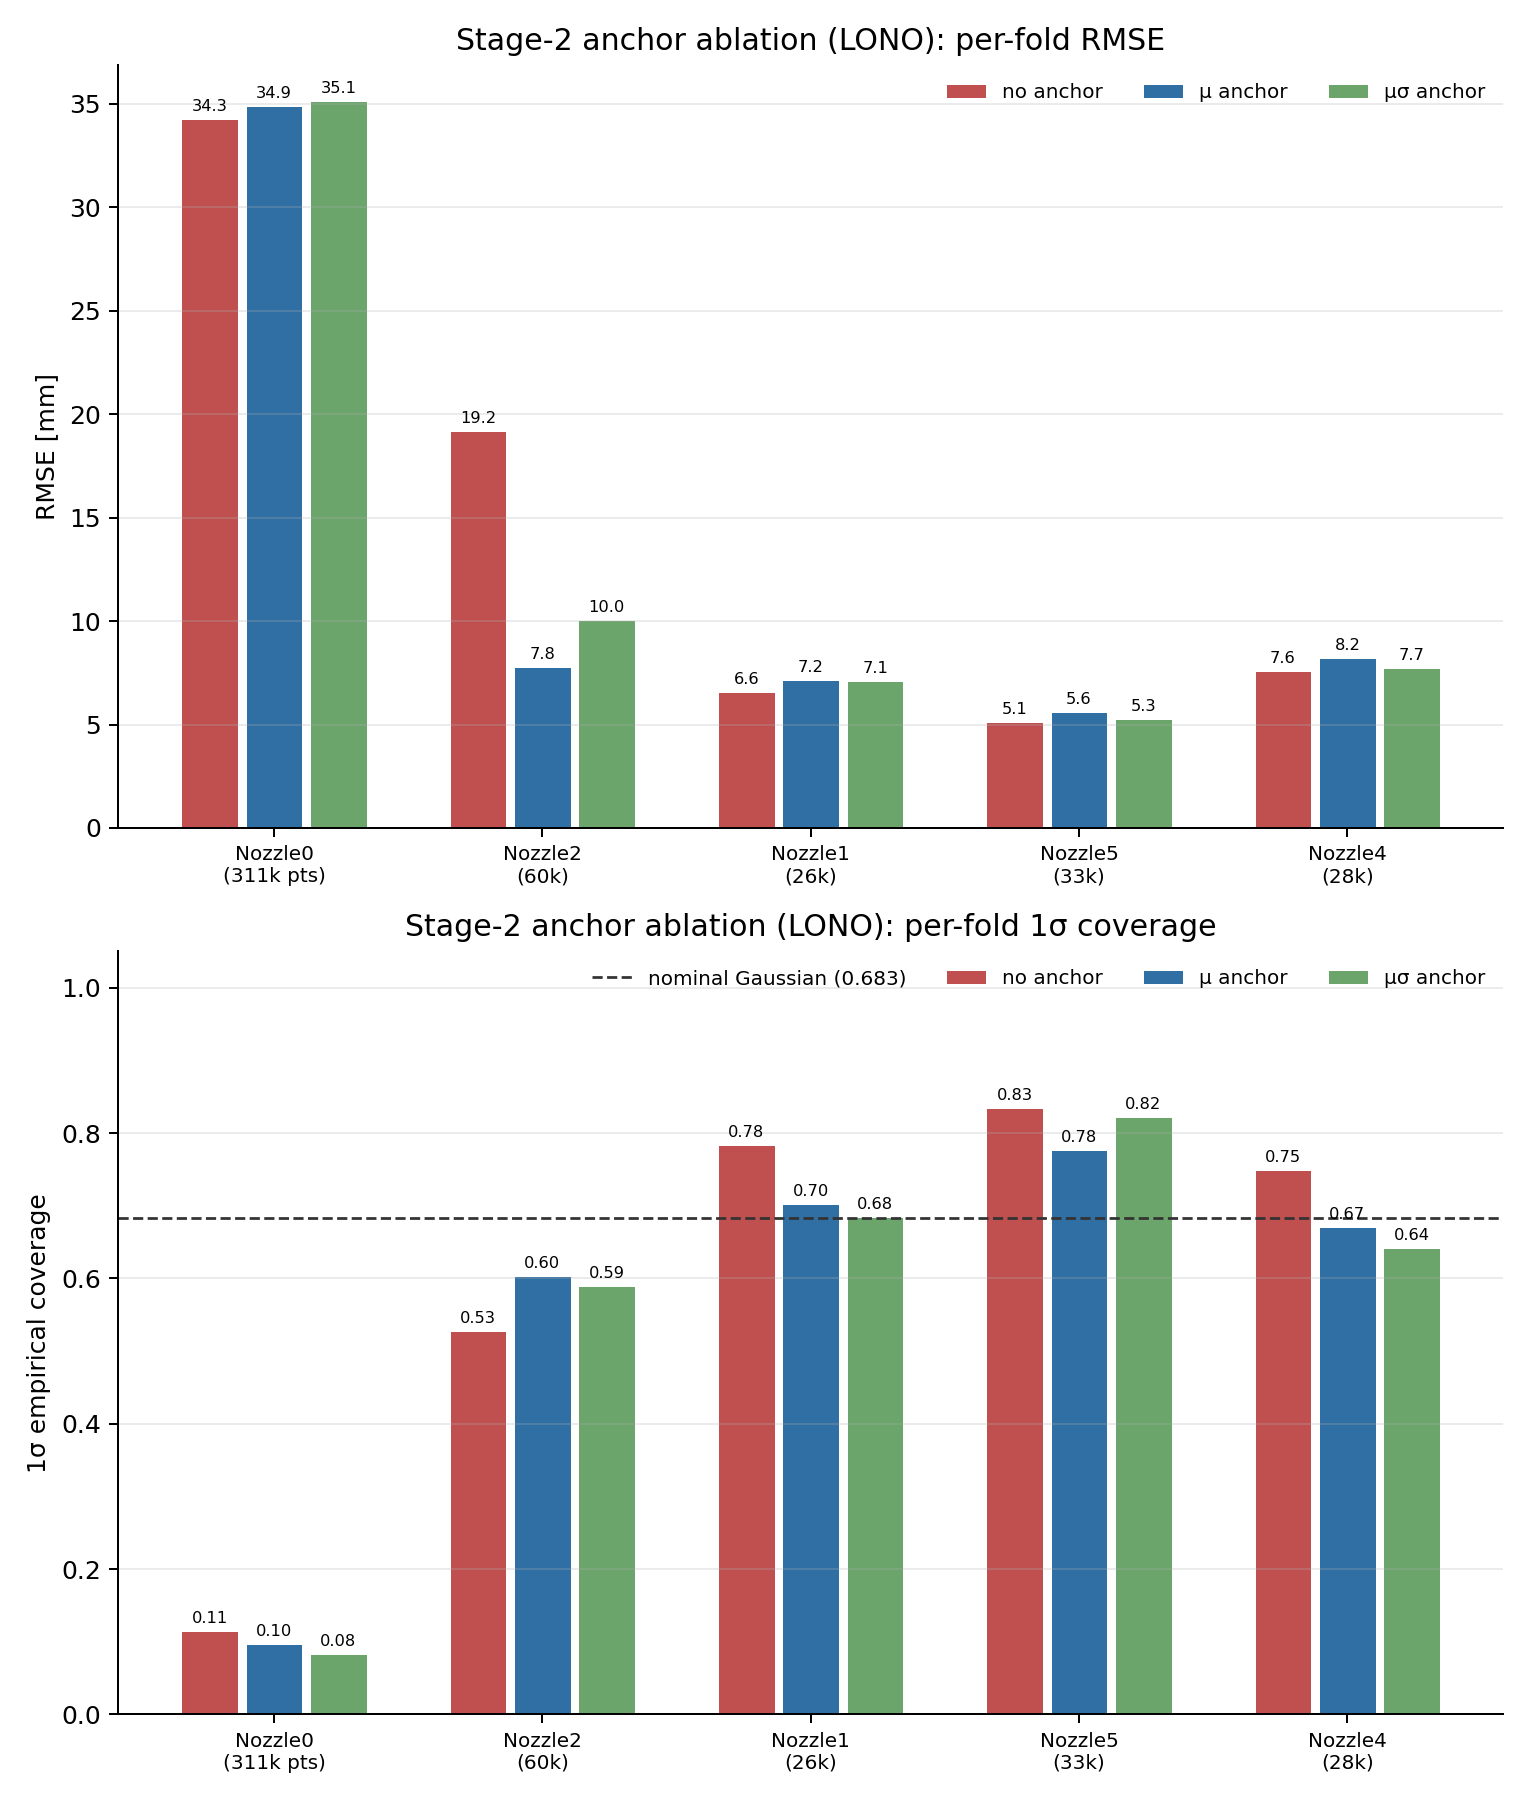
\includegraphics[width=\linewidth]{images/stage2_anchor_ablation.png}
\caption{阶段二 anchor 调度 LONO 消融总结。左：三种 anchor 变体的各折留出集 RMSE；右：各折 1$\sigma$ 覆盖率，虚线为名义高斯水平。源工件路径见附录~\ref{app:implementation_mapping}。}
\label{fig:stage2-anchor-ablation}
\end{figure}

该消融实验检验两个耦合的假设。首先，零时刻的均值 anchor 是否能在不造成其他位置条件均值偏差的代价下注入有用的物理先验；无 anchor 与仅 $\mu$-anchor 的对比孤立了这一权衡。其次，把早期 \(\sigma\) 强行压向其下限是否会损害对留出喷嘴族的不确定度标定；仅 $\mu$-anchor 与 $\mu$+$\sigma$ 双 anchor 的对比则把这一轴单独剥离开来，不受均值 anchor 的混杂影响。

两个假设的验证都指向支持仅 \(\mu\)-anchor 的结论。激活 \(\mu\)-anchor 会使平均 RMSE 降低 \SI{1.81}{mm}（从 14.54 降至 \SI{12.73}{mm}），MAE 降低 \SI{0.94}{mm}，2\(\sigma\) 覆盖率从 0.763 提升至 0.775，并将系统性低估偏差从 \SI{-8.50}{mm} 收窄至 \SI{-7.11}{mm}。改进主要集中在 Nozzle2 折：在没有 anchor 时，NLL 可以随意将数据稀少且靠近 \(t{=}0\) 的窗口用作松弛空间，导致无 anchor 在此处崩溃至 \SI{19.18}{mm} 的 RMSE；anchor 移除了这一自由度。这三个现代设计的喷嘴（Nozzle1/4/5，每折约 25k--33k 评估点）在三个变体下的结果彼此相差都在 \SI{1}{mm} 以内，可见 anchor 的价值只有在 LONO 折真正构成 OOD 挑战时才会显现。

在顶部叠加 \(\sigma\)-anchor 会把平均预测标准差从 \SI{5.68}{mm} 进一步收紧到 \SI{5.49}{mm}，但并未产生补偿性增益：RMSE 反而上升到 \SI{13.05}{mm} 且 2\(\sigma\) 覆盖率降至 0.764。这一现象可被解释为：将 \(\sigma\) 在 \(t{=}0\) 附近推向下限，会经由阶段三蒸馏传播为一种更自信但略带偏差的 \(\mu\) 预测，从而同时损害精度和标定。因此，下一小节报告的阶段三消融实验将阶段二教师固定在仅 $\mu$-anchor 配置下（\(\lambda_\mu=10^{-2}\)，\(\lambda_\sigma=0\)）；任何关于阶段三区制加权或 KD 形式的结论，都以该 anchor 选择为前提。完整的逐折明细与原始聚合文件归档路径见附录~\ref{app:implementation_mapping}。

\subsubsection{阶段三区制消融}

在阶段二 anchor 消融之后，本文将阶段二教师固定为仅 $\mu$-anchor 配置，并在同一五折 LONO 协议下重新运行阶段三的消融。该消融对比了四种阶段三配置：
(i)~\textbf{基准配置}，在可靠时间箱中设定 $w_{\mathrm{kd}}=0.25$ 且 $\lambda_{\mathrm{anchor}}=0.01$；
(ii)~\textbf{仅可靠区间纯原始变体}，移除可靠区间中的 KD 混合；
(iii)~\textbf{不确定区间混合变体}，在不确定区间中重新引入部分原始监督；以及
(iv)~\textbf{无锚点变体}，在保留 raw/KD 区制设计不变的同时设定 $\lambda_{\mathrm{anchor}}=0$。
表~\ref{tab:stage3-ablation-ranking} 提供了 LONO 排序。不确定区间混合变体取得了最低的平均 RMSE 和 MAE，而无锚点变体取得了最高的 2\(\sigma\) 覆盖率。各变体之间的差距较小：最佳和最差的平均 RMSE 仅相差 \SI{0.21}{mm}，远低于大约 \SI{12.5}{mm} 的跨折标准差。因此，这应当被解读为在阶段三调参上的微弱偏好，而不是决定性的架构级影响。

各折的模式解释了这个较小的总体差距。Nozzle0 对每个阶段三变体来说仍然是一个跨设计族的外推失败，RMSE 在 \SIrange{34.76}{35.31}{mm} 的范围内，并存在约 \(\approx\SI{-27}{mm}\) 的系统性低估偏差。不确定区间混合变体在 Nozzle2 和 Nozzle1 折上获胜，而基准配置在 Nozzle5 和 Nozzle4 折上获胜。因此，表~\ref{tab:stage3-ablation-ranking} 支持在固定阶段二仅 $\mu$-anchor 教师下将不确定区间混合变体作为 LONO 的 RMSE/MAE 胜出配置，但这并不构成对 70\%/20\% 覆盖率边界、\(\sigma_{\mathrm{ref}}=\SI{10}{mm}\) 或所有可能权重组合的全面超参数搜索。完整的运行工件归档路径见附录~\ref{app:implementation_mapping}。

\begin{table}[t]
\centering
\footnotesize
\begin{tabular}{lrrrrr}
\toprule
配置 & RMSE [mm] & MAE [mm] & Bias [mm] & 1$\sigma$ 覆盖率 & 2$\sigma$ 覆盖率 \\
\midrule
基准配置 & 12.68 $\pm$ 12.74 & 9.97 $\pm$ 10.55 & $-7.86 \pm 11.28$ & 0.565 & 0.759 \\
仅可靠区间纯原始变体 & 12.76 $\pm$ 12.48 & 10.01 $\pm$ 10.22 & $-7.45 \pm 11.35$ & 0.556 & 0.761 \\
\textbf{不确定区间混合变体} & \textbf{12.55 $\pm$ 12.46} & \textbf{9.80 $\pm$ 10.18} & \textbf{\boldmath$-6.87 \pm 11.53$} & \textbf{0.575} & 0.770 \\
无锚点变体 & 12.73 $\pm$ 12.44 & 9.86 $\pm$ 10.22 & $-7.11 \pm 11.51$ & 0.570 & \textbf{0.775} \\
\bottomrule
\end{tabular}
\caption{在固定阶段二教师为仅 $\mu$-anchor 后的阶段三 LONO 消融。每行报告五个留一喷嘴族的留出集均值~$\pm$~标准差。不确定区间混合变体在 RMSE/MAE 上获胜；无锚点变体的 2$\sigma$ 覆盖率最强。}
\label{tab:stage3-ablation-ranking}
\end{table}

消融趋势也阐明了为什么阶段三应被视为微调层，而非全面解决 OOD 喷嘴几何问题的方法。获胜的 LONO 变体并没有消除教师引导，只是修改了不确定区间内原始监督与 KD 的比例平衡，其主要优势体现在 Nozzle2 和 Nozzle1 上。相反，各变体之间 Nozzle0 几乎不变，证实了此处的主要失效是缺失设计族覆盖，而非阶段三区制时间表本身的问题。对于下游生产风格分析，这个 LONO 结果作为选择保守阶段三区制设置的证据，而下一节关于 KD 损失形式的研究则用于处理域内近 FOV 处的偏差机制。

\begin{figure}[t]
\centering
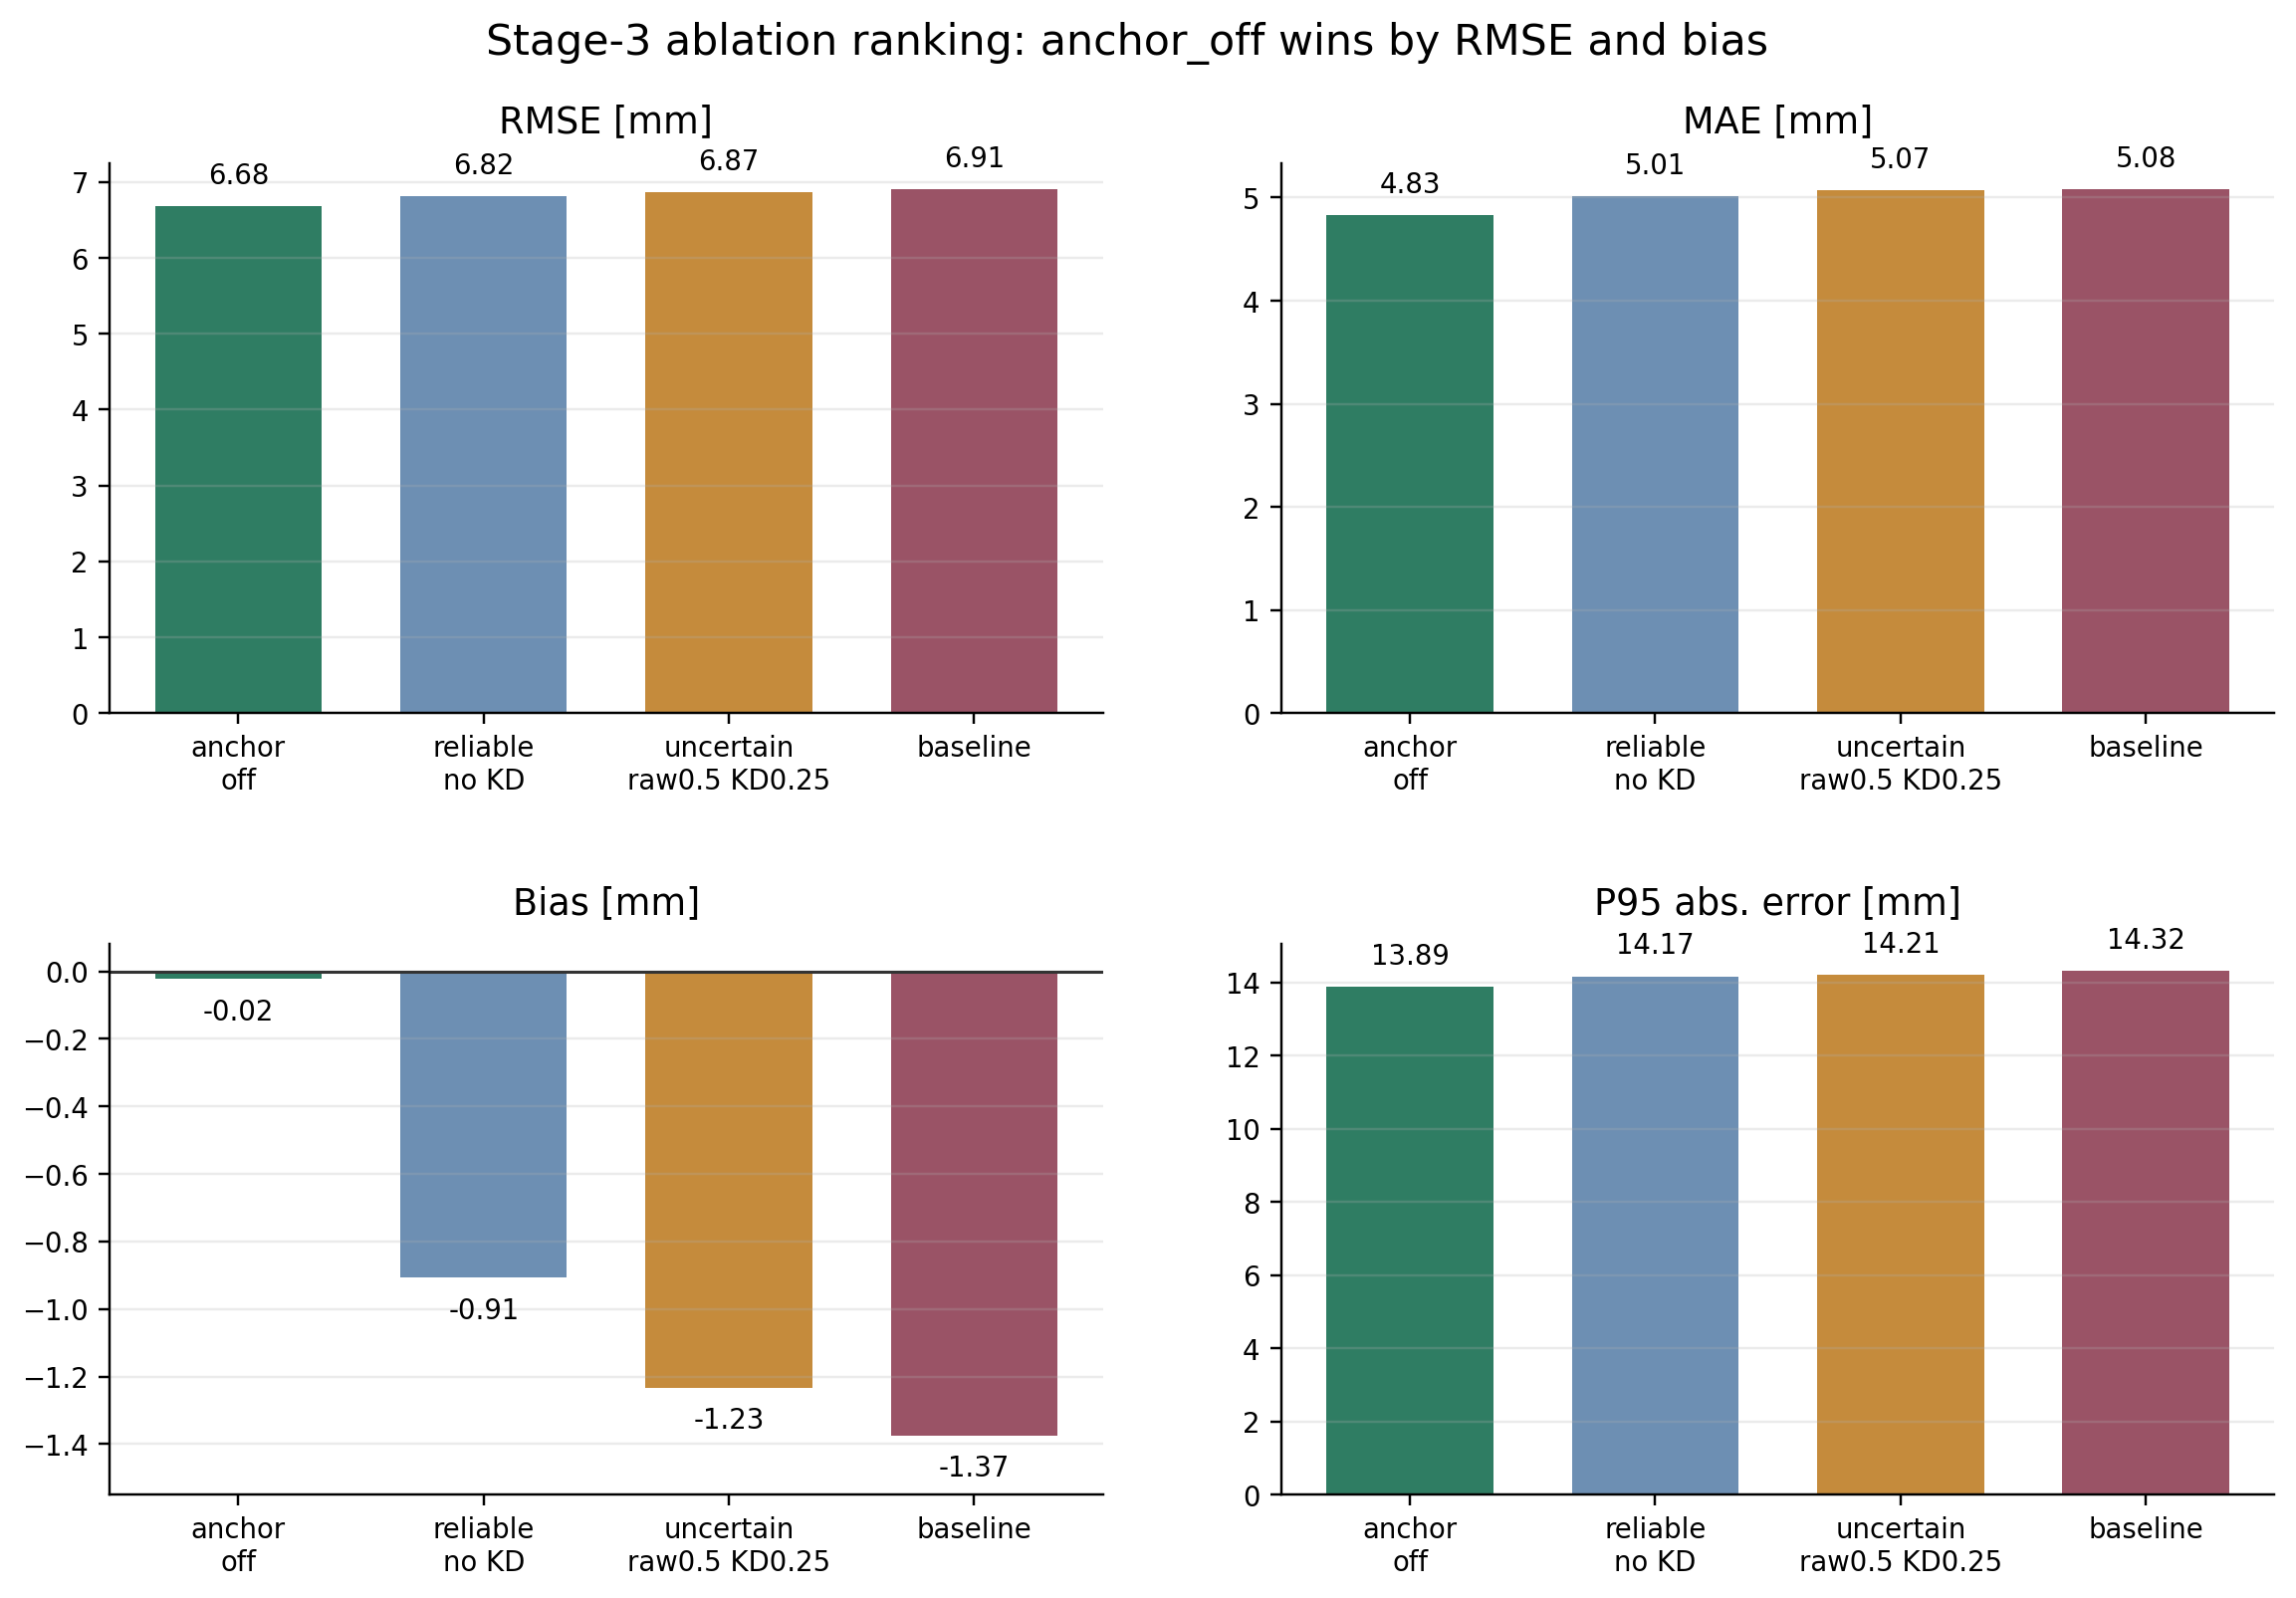
\includegraphics[width=\linewidth]{images/neural_network_fit_results/ablation_comparison_best.png}
\caption{阶段三 LONO 调参总结。在固定阶段二教师为仅 $\mu$-anchor 之后，不确定区间混合变体得到了最低的平均 RMSE/MAE，而无锚点变体提供了最强的 2$\sigma$ 覆盖率。源工件路径见附录~\ref{app:implementation_mapping}。}
\label{fig:ablation-best}
\end{figure}

\subsubsection{蒸馏损失形式的诊断与近 FOV 修复}
\label{sec:kd-form-fix-zh}

切换到将对数压力残差直接作为输入的"幅度缩放加压力残差"特征变体后，根据近视场指标 \(\mathrm{pen}\ge 0.9\,\mathrm{cap}_\mathrm{nozzle}\) 对阶段三的残差切片，暴露出高穿深区间中系统的性能下降：尽管阶段二教师在接近 FOV 顶部（cap）时几乎无偏（bias \SI{-0.59}{mm}，RMSE \SI{4.82}{mm}），但蒸馏出的无锚点学生在同一切片上的表现恶化为 bias \SI{-2.70}{mm} 且 RMSE 为 \SI{6.11}{mm}。这种漂移无法归因于阶段一/二的拟合——所采用的稳健清洗流程（Hampel 滤波与单调差分下界检测，详见 §3）在 cap 附近并未导致教师向下漂移——因此只可能由阶段三蒸馏步骤内部产生。

为定位机制，本文在保持上述教师不变的基础上，执行了七组单变量消融：关闭原始 NLL、关闭一阶/二阶形状惩罚、将 forward KL 中的置信度权重 \(\sigma_{\mathrm{ref}}/\sigma_{\mathrm{teacher}}\) 强制为 1、将 forward KL 替换为 reverse KL、使用仅 \(\mu\) 的 MSE 替换完整 KL、将训练缩短到 10 轮、以及将不确定与仅教师两个区制中的 KD 权重翻倍。其中两个变体较为突出：关闭原始 NLL 的诊断变体几乎精确重现了教师在近 cap 处的行为（bias \SI{-0.53}{mm}）；将完整 KL 替换为仅均值 MSE 的诊断变体把近 cap 偏差拉回至 \SI{-0.91}{mm}，并在所有变体中取得了全域最低 RMSE。二者指向两个共同原因：(i)~原始 NLL 把学生 \(\mu\) 拉向位于 FOV 顶部截断下一帧的下界观测值；(ii)~forward KL 项 \((\mu_t-\mu_s)^{2}/\sigma_s^{2}\) 允许学生仅靠膨胀自身的 \(\sigma\) 就可以逃避匹配教师 \(\mu\)。其余五个变体均把近 cap 偏差留在 \([-2.7,-2.0]\) mm 范围内，从而被排除为主要机制。

仅均值 MSE 的诊断变体切断了 \(\sigma\) 套利路径，但同时丢失了 KL 对学生 \(\sigma\) 的隐式监督，使得 KD-only 区间（不确定区间与仅教师区间）内的 \(\sigma\) 标定漂移。因此本文提出了均值 MSE 与对数方差 MSE 的混合蒸馏损失
\begin{equation}
\mathcal{L}_{\mathrm{KD}} \;=\; (\mu_s-\mu_t)^{2} \;+\; \lambda_\sigma\,\bigl(\log\sigma_s^{2} - \log\sigma_t^{2}\bigr)^{2},
\label{eq:kd-mse-mu-plus-sigma}
\end{equation}
即在均值 MSE 之上增加一个显式的对数方差 MSE，使 \(\sigma\) 重新受到监督，但同时避免重新引入 KL 形式所允许的 \(\sigma\)-套利。通过对 \(\lambda_\sigma\in\{0.5,1,2,5\}\) 进行扫描，选定 \(\lambda_\sigma=5.0\) 作为阶段三新默认值：在此设置下，近 cap 处的 RMSE 和 bias 达到联合最佳（\SI{4.89}{mm} 与 \SI{-0.66}{mm}），统计上与教师的 \(\SI{-0.59}{mm}\) 无法区分；同时在仅教师区间切片上逐点 \(|\sigma_s-\sigma_t|\) 中位值降至 \SI{0.27}{mm}。图~\ref{fig:kd-overlay} 叠加了教师、基准 forward-KL 学生与新混合蒸馏学生的偏差--真值曲线；改善主要集中在穿深的较高区间，下半段保持未受干扰。

\begin{figure}[t]
\centering
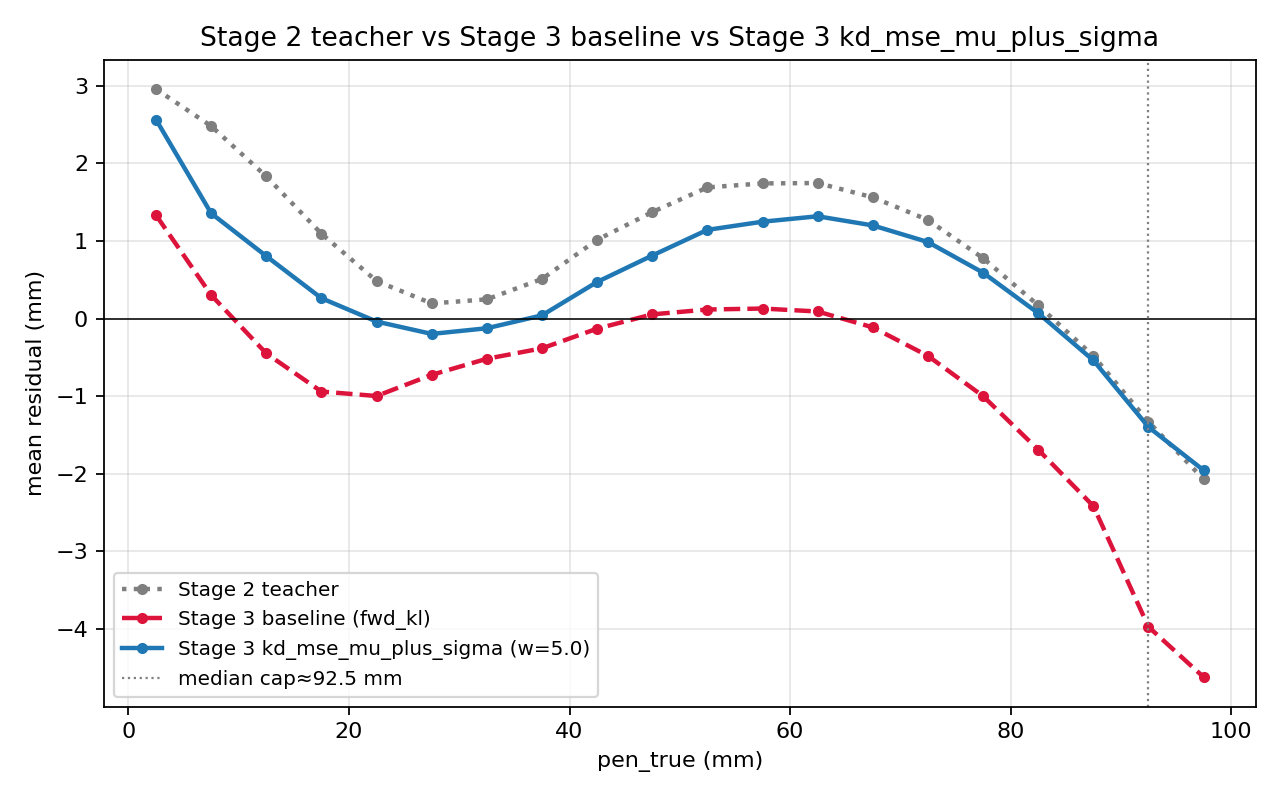
\includegraphics[width=0.82\linewidth]{images/neural_network_fit_results/stage3_kd_mse_mu_plus_sigma_overlay_baseline.png}
\caption{阶段三蒸馏损失形式对 bias--truth 曲线的影响。阶段二教师在 FOV cap 附近几乎无偏；基准 forward-KL 蒸馏在近 cap 处引入了大约 \(\approx -2.7\,\mathrm{mm}\) 的额外下偏；本文混合蒸馏损失（\(\lambda_\sigma=5\)）将曲线拉回贴近教师。曲线表示 \SI{5}{mm} 真值箱中的平均残差。}
\label{fig:kd-overlay}
\end{figure}

由于阶段三在三种不同的监督区制上训练，按区制分别汇报留出集评估比单独汇总更合适。固定阶段一、二的前提下在五个随机种子 \(\{7,17,42,99,2024\}\) 上重训练阶段三（即"模式 A"协议），最终混合蒸馏模型（\(\lambda_\sigma=5.0\)）在每个种子的 692{,}942 个留出时间点上取得了总体 RMSE \(\SI{4.735}{mm}\pm\SI{0.037}{mm}\)、MAE \(\SI{3.293}{mm}\pm\SI{0.039}{mm}\) 与偏向 \(\SI{+0.626}{mm}\pm\SI{0.112}{mm}\) 的全净化成绩。若将同样的五种子评估限制在保守的未删失 CDF 子集（在去除高密度分布及 FOV 饱和截断后包含 \num{542565} 个点）上，则得到 RMSE \(\SI{4.265}{mm}\pm\SI{0.040}{mm}\)、MAE \(\SI{3.032}{mm}\pm\SI{0.048}{mm}\)、偏向 \(\SI{+0.562}{mm}\pm\SI{0.119}{mm}\)，以及 1\(\sigma\)/2\(\sigma\) 覆盖率分别为 \(0.887\pm 0.004\) / \(0.989\pm 0.001\)（各种子具体数值与归档路径见附录~\ref{app:implementation_mapping}）。表~\ref{tab:stage3-kd-regimes} 按训练时的监督区制与 FOV 删失标志分别给出详细指标（数值取自代表性种子 \(s=99\)）。可靠区间切片（占样本 79\%）受原始 NLL 监督主导，RMSE 为 \SI{4.68}{mm}、bias 为 \SI{+0.67}{mm}；KD-only 切片（合并不确定与仅教师两区间，占 21\%）RMSE 为 \SI{5.08}{mm}、bias 为 \SI{+0.93}{mm}，虽稍高但仍优于此前基准的全域聚合。通过 FOV 删失视角看：未发生 FOV 截断的轨迹（n=393{,}912）RMSE \SI{4.85}{mm}、bias \SI{+0.99}{mm}；发生截断的轨迹（n=299{,}030）RMSE \SI{4.65}{mm}、bias \SI{+0.37}{mm}；二者交集即右删失轨迹中的近 cap 点（n=47{,}676）达到 RMSE \SI{4.95}{mm}、bias \SI{-0.69}{mm}，与教师在同一切片上的 \SI{-0.59}{mm} 实质匹配。全部五个种子的整体近 cap 切片 RMSE 为 \(\SI{4.881}{mm}\pm\SI{0.024}{mm}\)，bias 为 \(\SI{-0.566}{mm}\pm\SI{0.079}{mm}\)；右删失轨迹中的近 cap 点切片 RMSE 为 \(\SI{4.939}{mm}\pm\SI{0.023}{mm}\)，bias 为 \(\SI{-0.590}{mm}\pm\SI{0.077}{mm}\)。\(-0.590\,\si{mm}\) 与教师同切片 \SI{-0.59}{mm} 之间的差异小于单个种子标准差，这证实蒸馏诱发的失真已被修复且对随机初始化稳健。

\begin{figure}[t]
\centering
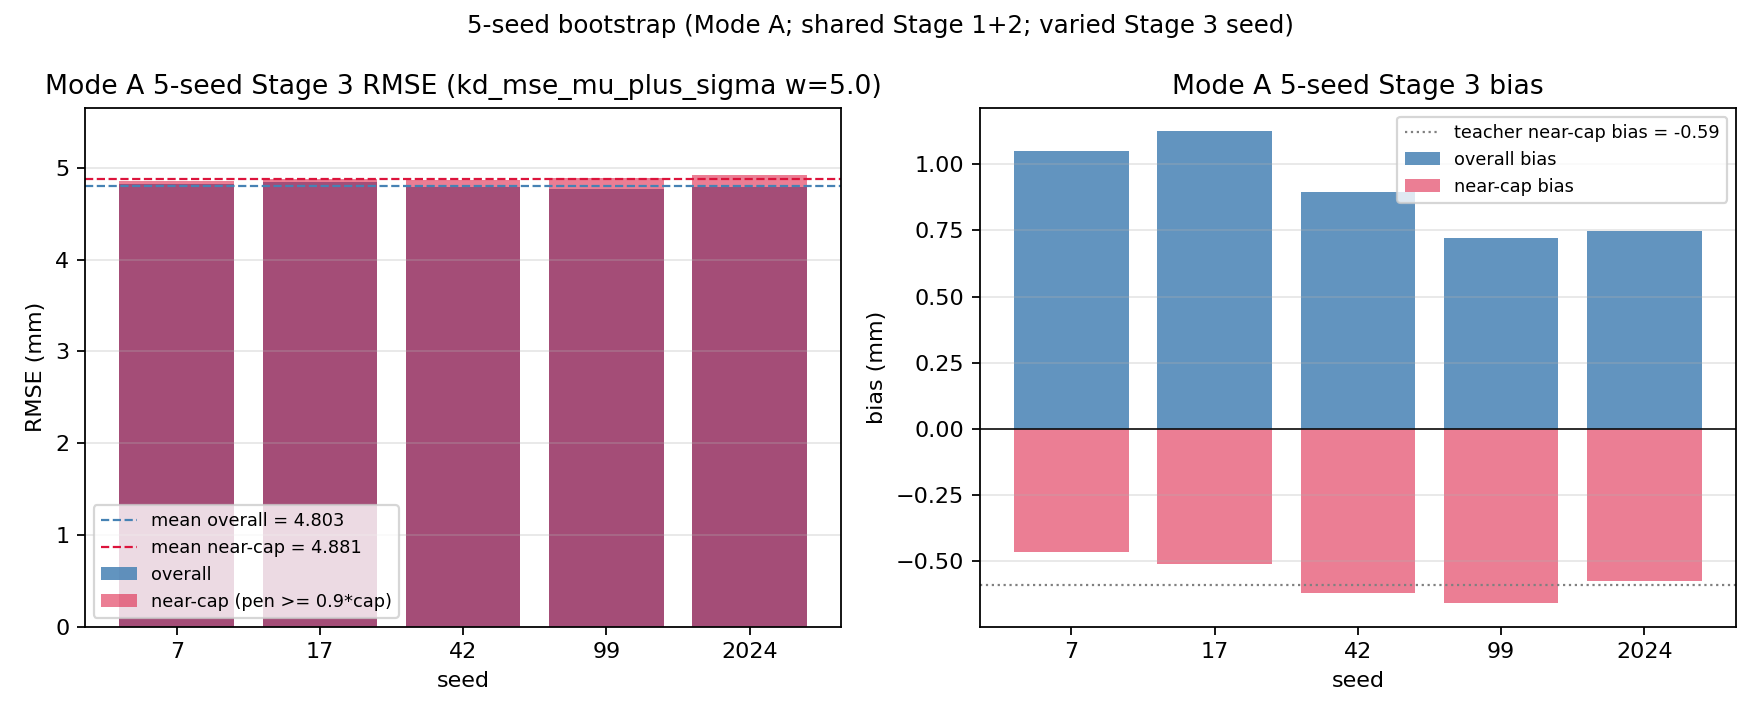
\includegraphics[width=0.95\linewidth]{images/neural_network_fit_results/stage3_kd_mse_mu_plus_sigma_modeA_per_seed.png}
\caption{在模式 A 协议下（共享阶段一+二，五个种子 \(\{7,17,42,99,2024\}\)）的逐种子阶段三表现。左：留出集 RMSE，整体与近 cap 切片（\(\mathrm{pen}\ge 0.9\,\mathrm{cap}\)）并列显示；虚线标示五次运行的均值。右：对应的 bias 值；灰色点线表示阶段二教师的近 cap bias \SI{-0.59}{mm}。RMSE 标准差为 \SI{0.032}{mm}（相对 0.7\%），近 cap bias 标准差为 \SI{0.079}{mm}，证实蒸馏结果在不同随机初始化下稳健。}
\label{fig:kd-modeA-per-seed}
\end{figure}

\begin{table}[t]
\centering
\small
\begin{tabular}{lrrrr}
\toprule
切片 & n & RMSE [mm] & Bias [mm] & 中位 \(|\sigma_s-\sigma_t|\) [mm] \\
\midrule
全集 & 692{,}942 & 4.76 & +0.72 & 0.82 \\
可靠原始区间 & 549{,}299 & 4.68 & +0.67 & 1.00 \\
不确定原始区间 & 64{,}487 & 5.88 & +1.27 & 0.40 \\
仅教师区间 & 79{,}156 & 4.33 & +0.65 & \textbf{0.27} \\
KD-only（合并） & 143{,}643 & 5.08 & +0.93 & 0.32 \\
近 cap (\(\mathrm{pen}\ge 0.9\,\mathrm{cap}\)) & 54{,}704 & 4.89 & \(-\)0.66 & 0.27 \\
轨迹未删失 & 393{,}912 & 4.85 & +0.99 & 0.81 \\
轨迹删失 & 299{,}030 & 4.65 & +0.37 & 0.84 \\
轨迹删失 \& 近 cap & 47{,}676 & 4.95 & \(-\)0.69 & 0.28 \\
\bottomrule
\end{tabular}
\caption{混合蒸馏模型（\(\lambda_\sigma=5.0\)）的各切片留出集指标。"可靠原始区间"表示由原始 NLL 主导的监督区域；"KD-only"合并了不确定原始区间和仅教师区间，均完全受 Eq.~\eqref{eq:kd-mse-mu-plus-sigma} 监督。中位 \(|\sigma_s-\sigma_t|\) 逐点比对阶段二教师的 \(\sigma\) 计算，用以量化标定漂移程度。}
\label{tab:stage3-kd-regimes}
\end{table}

\begin{figure}[t]
\centering
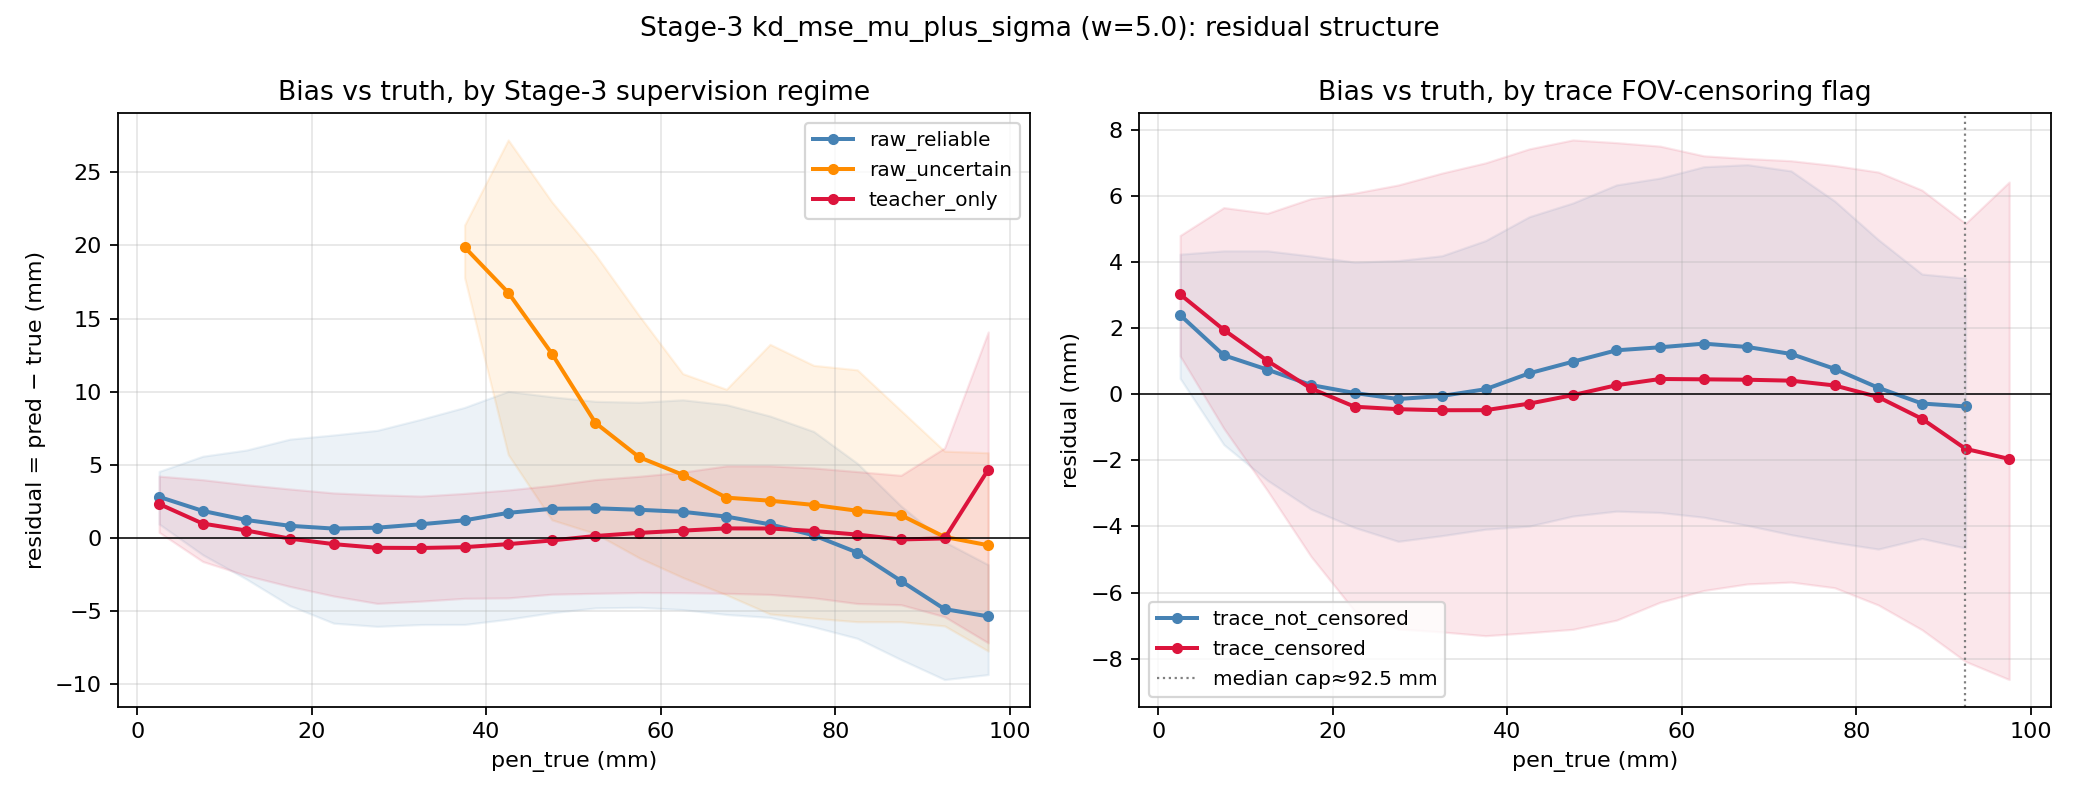
\includegraphics[width=\linewidth]{images/neural_network_fit_results/stage3_kd_mse_mu_plus_sigma_residual_vs_truth.png}
\caption{混合蒸馏模型（\(\lambda_\sigma=5\)）的残差结构。左：按训练区制分类（可靠原始区间 / 不确定原始区间 / 仅教师区间）；右：按轨迹级 FOV 删失标志分类。阴影区域表示 P10--P90 的残差范围。}
\label{fig:kd-residual-by-regime}
\end{figure}

\begin{figure}[t]
\centering
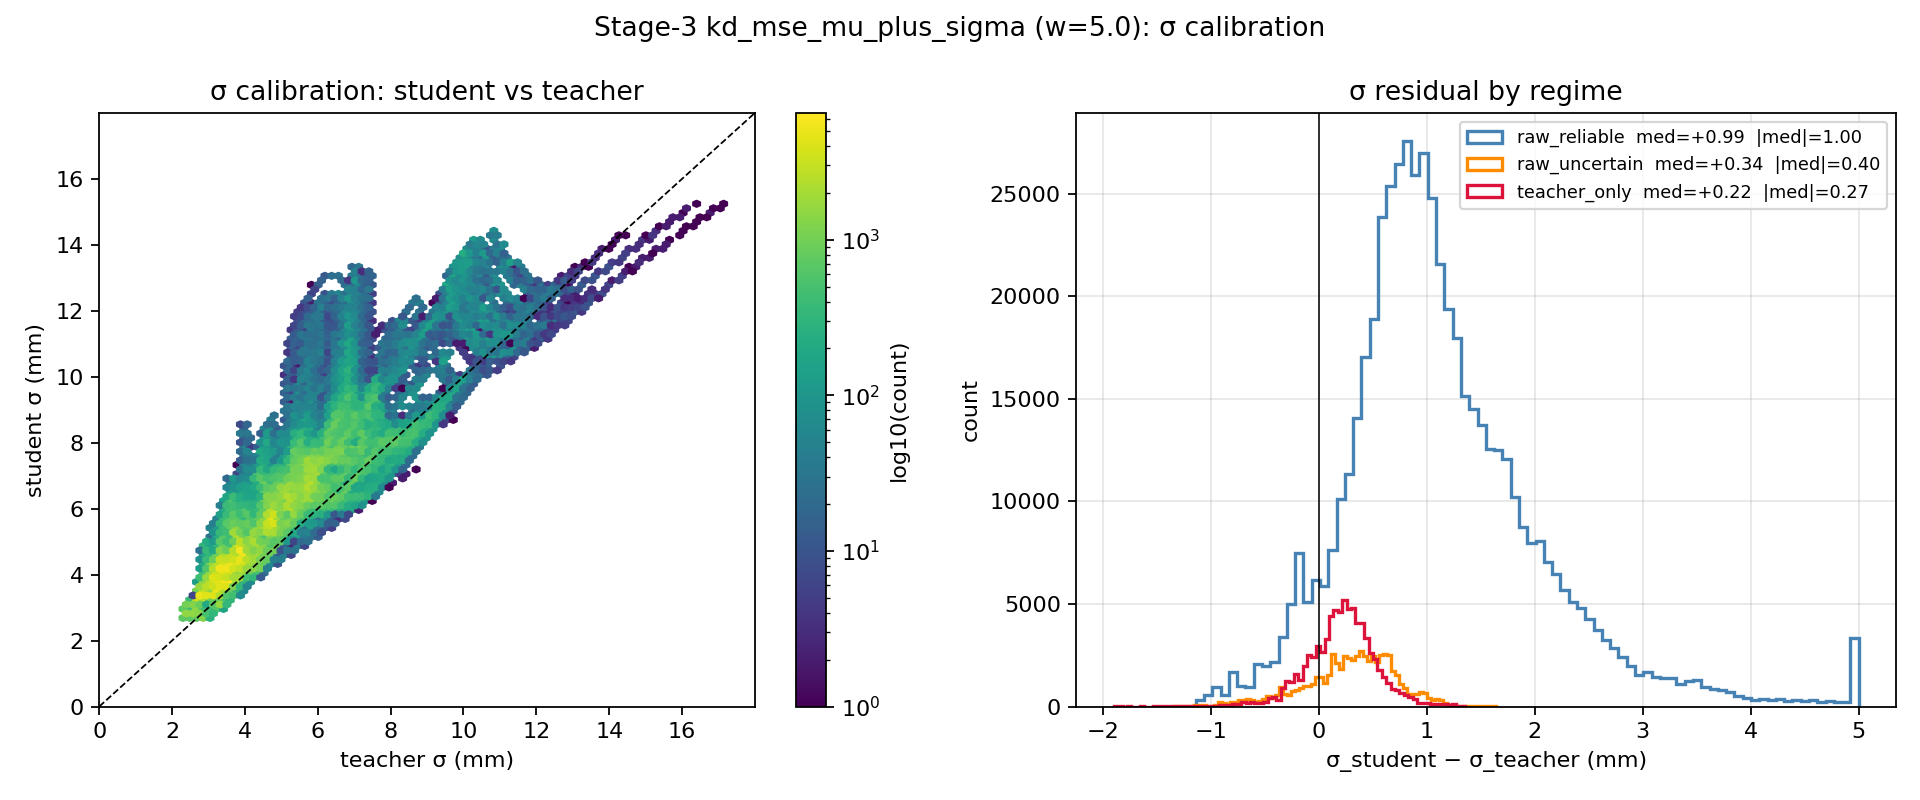
\includegraphics[width=\linewidth]{images/neural_network_fit_results/stage3_kd_mse_mu_plus_sigma_sigma_calibration.png}
\caption{混合蒸馏模型（\(\lambda_\sigma=5\)）的不确定度标定情况。左：学生 \(\sigma\) 对教师 \(\sigma\) 的逐点六边形热力联合分布；右：各监督区制下残差 \(\sigma_s-\sigma_t\) 的分布直方图。}
\label{fig:kd-sigma-calibration}
\end{figure}

\subsubsection{方法论补充：消融可负担性作为 MLP 架构的特有优势}
\label{sec:mlp-ablation-affordability-zh}

选择 MLP 作为穿深代理模型架构的一个直接结果，是本文所报告的系统化消融在普通硬件上计算可负担。本文中独立的消融矩阵共有三组：阶段一在 9 个工程化特征变体上的 5 折 LONO（第~\ref{sec:stage1-lono-ablation-zh} 小节）、阶段二在 3 种 anchor schedule 上的同协议 LONO 对比、以及阶段三在 4 种区制加权变体与 7 组单变量 KD 形式消融上的组合搜索。支持头表所需的完整 LONO~$\times$~消融~$\times$~种子网格，在单张消费级加速器上大约消耗数十 GPU 小时。

更核心的论证不在单次训练耗时，而在任务结构与架构归纳偏置的匹配关系。本文代理模型的目标是把 $(\mu,\sigma)$ 作为低维工况描述子（时间、缩放后的幅值、对数压力残差、喷嘴族独热指示）的逐点函数进行回归，输入既无规则空间网格、也无长程序列依赖。激发 CNN 设计的局部平移不变性偏置和驱动 Transformer 的长程注意力偏置都与此种逐点低维回归任务结构不匹配；两者会引入任务并不需要的表达能力与参数量。在此基础上，本文设计归因所要求的特征工程、anchor schedule、区制权重、KD 损失形式的组合扫描——共数十种配置~$\times$~五折 LONO~$\times$~多个种子——需要在每个变体上独立完整训练；引入更复杂的时空主干会同时放大单次成本与可比配置数量，结果是硕士级别算力预算下只能报告单一配置而无法分离各设计选择的边际贡献。因此，架构-任务匹配与消融可负担性共同使 MLP 成为有原则性的选择，而不是仅仅为省事而做出的权宜之计；本文第~4 章与第~5 章呈现的系统化消融证据，若没有这种匹配，在硕士级别算力预算下是无法触及的。这一定性结论不依赖对 CNN/Transformer 训练成本的具体数值断言，本文也未对此进行直接基准测试。

\subsubsection{原型筛查输出与证据边界}

最终 surrogate 可以与一个简化的碰壁筛查几何耦合。当前的 GUI 原型使用 MLP，因为它已经暴露出时间筛查显示所需的喷射起始（onset）辅助输出；SVGP 可以替代穿深的 $\mu,\sigma$ 通道，但它本身不能直接替代该起始预测头。在默认的玩具输入下：
\[
\left\{
\begin{aligned}
d_n &= \SI{0.34}{mm},\\
p_{\mathrm{inj}} &= \SI{2000}{bar},\\
p_{\mathrm{amb}} &= \SI{15}{bar},\\
\theta_{\mathrm{tilt}} &= 20^{\circ},\\
N_{\mathrm{plume}} &= 10,\\
t_{\mathrm{inj}} &= \SI{800}{\micro s},\\
\mathrm{RPM} &= 250,
\end{aligned}
\right.
\]
原型在 0--\SI{5}{ms} 窗口内生成了用于绘图的非负均值 $\mu_{+}(t)\in[\SI{1.70}{mm},\,\SI{112.95}{mm}]$ 和 $\sigma_{\parallel}(t)\in[\SI{4.39}{mm},\,\SI{17.66}{mm}]$。瞬时近壁截获分数在 $t=\SI{4.237}{ms}$ 时达到峰值 $P_{\mathrm{hit}}=\SI{77.66}{\percent}$，梯形积分得到的累积暴露量为 $E=\SI{2.475}{ms}$。这些数值说明，端到端链路已经能够将穿深分布转化为时间分辨的筛查分数；图~\ref{fig:impingement-preview-zh} 给出峰值时刻的空间快照，图~\ref{fig:impingement-summary-zh} 总结了 \SI{5}{ms} 窗口内的概率时间历程。

\begin{figure}[t]
\centering
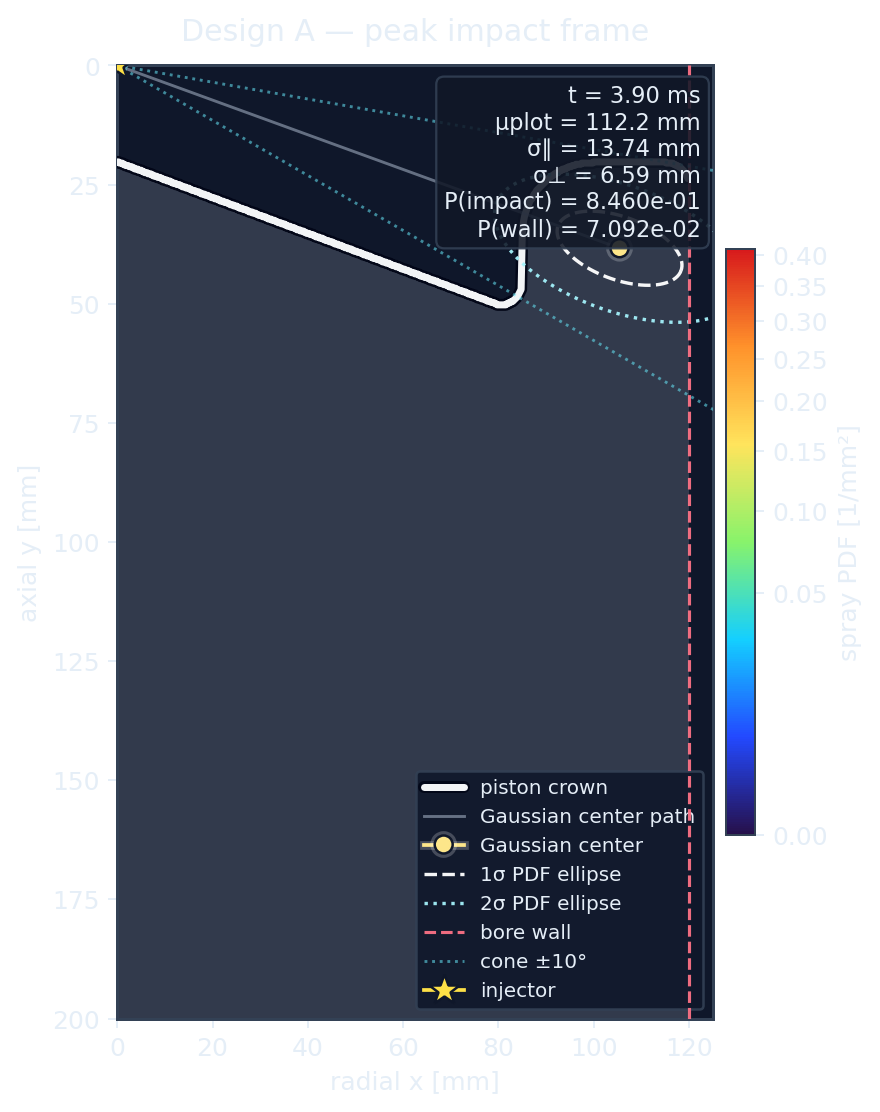
\includegraphics[width=0.62\linewidth]{images/impingement_preview.png}
\caption{碰壁筛查原型的空间快照（Design A，峰值碰撞帧，$t=\SI{4.24}{ms}$）。白色实线为活塞顶轮廓，红色虚线为缸壁，金色星号为喷嘴位置，白色虚线椭圆和青色点线椭圆分别为喷雾二维高斯密度的 $1\sigma$ 与 $2\sigma$ 等值线，色条表示喷雾概率密度（$\si{mm^{-2}}$）。该帧的瞬时活塞截获概率为 $P_{\mathrm{hit}}=\SI{77.66}{\percent}$，缸壁截获概率为 $P_{\mathrm{wall}}=\SI{6.60}{\percent}$。}
\label{fig:impingement-preview-zh}
\end{figure}

\begin{figure}[t]
\centering
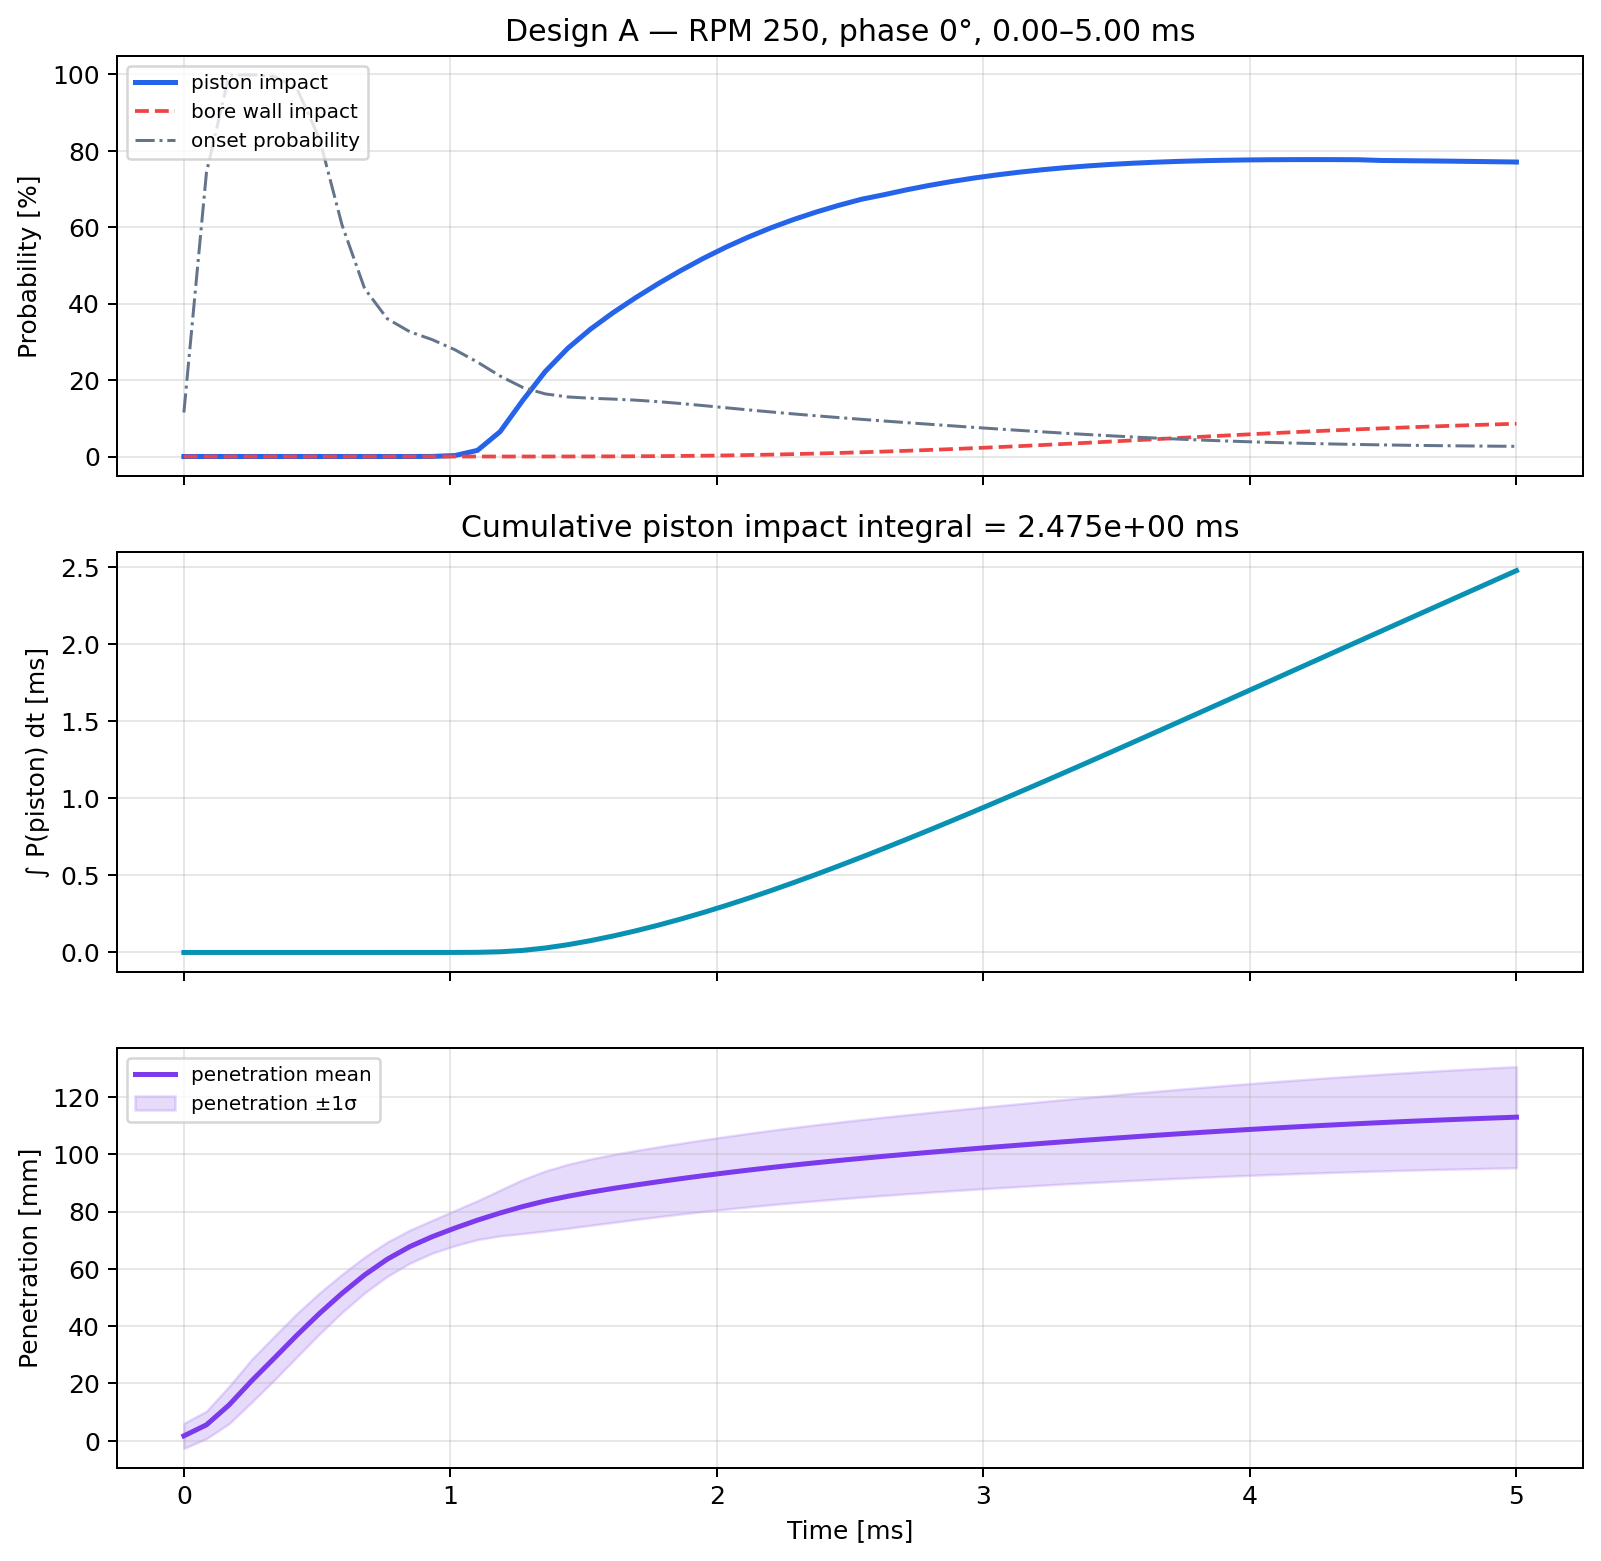
\includegraphics[width=0.90\linewidth]{images/impingement_summary.png}
\caption{碰壁筛查原型的时间总结（Design A，转速 RPM~250，曲轴相位 $0^{\circ}$，$0$--$\SI{5}{ms}$）。上图为瞬时截获概率：蓝色实线为活塞碰撞概率，红色虚线为缸壁碰撞概率，蓝灰色点划线为喷射起始概率的辅助输出。中图为活塞截获概率的时间累积积分 $E=\int P_{\mathrm{hit}}\,\mathrm{d}t$，在 $\SI{5}{ms}$ 时达到 $\SI{2.475}{ms}$。下图为穿深均值及其 $\pm1\sigma$ 区间。}
\label{fig:impingement-summary-zh}
\end{figure}

证据边界同样重要。上述碰撞概率只应被解读为管道的演示和面向排名的代理指标，不能直接等同于真实发动机中发生有害液态撞壁的实际概率。本文验证过的贡献是其测量范围内的穿深 surrogate 以及它与概率几何筛查接口的耦合，而不是对有害液态撞壁进行相态分辨的预测器。本文报告的数值声明均可追溯至清洗后的轨迹表、保存的检查点，以及项目归档中所包含的导出评估图。
